\documentclass[11pt,letterpaper]{article}

\usepackage[margin=1.18in]{geometry}
\usepackage[T1]{fontenc}
\usepackage[utf8]{inputenc}
\usepackage{lmodern}
\usepackage{microtype}
\usepackage{amsmath,amssymb,mathtools}
\usepackage{booktabs}
\usepackage{longtable}
\usepackage{array}
\usepackage{xcolor}
\usepackage{tikz}
\usetikzlibrary{positioning,arrows.meta,calc}
\usepackage{fancyhdr}
\usepackage{titlesec}
\usepackage{enumitem}
\usepackage[colorlinks=true]{hyperref}

\definecolor{headblue}{RGB}{31,73,125}
\definecolor{linkblue}{RGB}{42,92,141}
\hypersetup{linkcolor=headblue,citecolor=linkblue,urlcolor=linkblue,
  pdftitle={Recursive Spectral Fibers on Simplicial Cobordisms},
  pdfauthor={Tessera - cobordism programme},
  pdfsubject={Recursive spectral fibers on simplicial cobordisms}}

\definecolor{estblue}{RGB}{230,238,248}
\definecolor{estblueline}{RGB}{90,124,160}
\definecolor{derivgreen}{RGB}{232,244,233}
\definecolor{derivgreenline}{RGB}{96,140,100}
\definecolor{propamber}{RGB}{253,244,227}
\definecolor{propamberline}{RGB}{188,136,54}
\definecolor{firewallred}{RGB}{176,48,42}

\titleformat{\section}{\Large\bfseries\sffamily\color{headblue}}{\thesection}{0.7em}{}
\titleformat{\subsection}{\large\bfseries\sffamily\color{headblue}}{\thesubsection}{0.7em}{}

\pagestyle{fancy}
\fancyhf{}
\fancyhead[L]{\small\sffamily Recursive Spectral Fibers}
\fancyhead[R]{\small\sffamily Tessera}
\fancyfoot[C]{\small\thepage}
\renewcommand{\headrulewidth}{0.4pt}

\newcommand{\code}[1]{\texttt{#1}}
\newcommand{\dG}{d\Gamma}
\newcommand{\Fock}{\mathcal{F}_{-}}
\newcommand{\hh}{\mathfrak{h}}
\newcommand{\HK}{\mathcal{H}}
\newcommand{\RN}{\mathcal{R}}
\newcommand{\gtens}{\mathbin{\widehat{\otimes}}}
\newcommand{\su}{\mathfrak{su}}
\newcommand{\lsum}{\mathbin{\boxplus}}

\setlist[itemize]{topsep=2pt,itemsep=2pt,parsep=0pt}
\setlist[enumerate]{topsep=2pt,itemsep=2pt,parsep=0pt}

\tikzset{
  estbox/.style={draw=estblueline,fill=estblue,rounded corners=1.5pt,align=center,font=\small\sffamily,inner sep=5pt},
  derivbox/.style={draw=derivgreenline,fill=derivgreen,rounded corners=1.5pt,align=center,font=\small\sffamily,inner sep=5pt},
  propbox/.style={draw=propamberline,fill=propamber,rounded corners=1.5pt,align=center,font=\small\sffamily,inner sep=5pt},
  flow/.style={-{Stealth[length=2.6mm]},semithick,draw=black!60},
}

\begin{document}
\hypersetup{pageanchor=false}

% ---------------------------------------------------------------- title
\begin{titlepage}
\begin{center}
\vspace*{1.1cm}
{\LARGE Recursive Spectral Fibers on Simplicial Cobordisms\par}
\vspace{0.4cm}
{\large A geometric program for quarks, color, fermion statistics, Fock space, and baryons\par}
\vspace{0.9cm}
{\large Tessera -- cobordism programme\par}
\vspace{0.7cm}
{\small\color{linkblue} Implementation is tracked by GitHub epic \#763.\par}
\vspace{0.4cm}
{\bfseries Abstract\par}
\end{center}
\begingroup\small

\noindent
This paper proposes a single geometric formulation for the particle content
already suggested by Tessera's cobordism experiments. A persistent, spectrally
certified connected simplicial component is treated as one effective vertex at
the next resolution. The component's selected localized Hodge eigenspace is its
fiber, and the couplings between components induce transport between those
fibers. Repeating this operation produces a nested, potentially fractal
hierarchy of complexes. No independent gauge field, particle label, or
auxiliary lattice is introduced. Each edge supplies one two-level occupation
mode and complex geometric data, while the generally entangled state lives on
the exterior Fock space of all active edge modes. Connections, exchange signs,
and observables are derived from that state and the Hodge/Regge operators
already present in the construction.

\medskip
\noindent
The proposal has a substantial exact core. Static Schur reduction proves when a
component may be replaced by a response vertex without changing supported
boundary quadratic energies. Nonzero spectral bands instead use the
energy-dependent Feshbach--Schur map, or a certified Craig--Bampton/AMLS linear
surrogate. Simplicial gluing acts on the one-particle chain space; fermionic
second quantization then turns direct sums into graded tensor products and
coupling blocks into hopping terms. Every generator so obtained is quadratic,
so the dynamics is exactly quasi-free: the state is carried without loss by a
covariance matrix, Wick's theorem evaluates every polynomial certificate, and
mean-field geometry backreaction provably stays Gaussian. Three oriented
edge-mode factors form the
exact exterior algebra $\Lambda^{\bullet}\mathbb{C}^{3}=\mathbf{1}\oplus
\mathbf{3}\oplus\overline{\mathbf{3}}\oplus\mathbf{1}$; the one-occupation
sector is a color qutrit, its bilinears close $\su(3)$, the three-occupation
sector is a color singlet, and the grading gives the fermionic exchange sign
and canonical anticommutation relations. A rank-$r$ connection is derived from
overlap of neighboring spectral frames. At rank three its determinant line and
projective $SU(3)/\mathbb{Z}_{3}$ transport are retained rather than choosing
an unrecorded cube-root branch. Closed holonomies are gauge-invariant
observables rather than new degrees of freedom. Successive cobordism
interactions generate the finite stages of an inductive-limit Fock space.

\medskip
\noindent
The physical identification remains a hypothesis to be tested. A quark is
proposed to be a persistent, odd-parity, rank-three spectral fiber anchored to
oriented faces of a certified component; a proton is three such components
bound into one persistent supercomponent, occupying a normalized color wedge,
carrying baryon number \code{+1}, electric charge \code{+1}, and a
sharpness-certified total-space spin-\code{1/2} readout. The paper separates
exact identities, results already supported by Tessera, and new falsifiable
conjectures, and it states the sharpest open question as a dichotomy: either an
exact covariance-only proton exists, or a genuinely non-Gaussian,
geometry-mediated interaction is required. An implementation program of
structure-exact operations before iterative numerics keeps the defining
observables from becoming uncontrolled approximations.
\endgroup
\end{titlepage}

% ---------------------------------------------------------------- TOC
\hypersetup{pageanchor=true}
\pagenumbering{roman}
\tableofcontents
\clearpage
\pagenumbering{arabic}

% ================================================================ 1
\section{Epistemic status and design constraint}\label{sec:epistemic}

Three kinds of statement are deliberately distinguished:
\begin{enumerate}
  \item \textbf{Exact identity} --- follows algebraically from the stated
    finite complex, orientation, and inner product.
  \item \textbf{Existing Tessera evidence} --- measured by an existing
    experiment, with the scope and residual reported in the repository.
  \item \textbf{Proposed physical identification} --- a new hypothesis with an
    explicit falsification test.
\end{enumerate}

The governing constraint is parsimony. The ontology is limited to:
\begin{itemize}
  \item an oriented simplicial complex and its cobordisms;
  \item on each edge, a complex squared length and a complex
    $\mathbb{C}^{*}$ connection phase --- two distinct fields, because the
    connection is gauge-variant and the geometry is not --- together with one
    two-level occupation mode;
  \item incidence, Hodge, and Regge operators derived from that data;
  \item a generally entangled boundary/Fock state on those modes; and
  \item simplicial gluing followed by fermionic second quantization.
\end{itemize}

Spectral fibers, color frames, connections, Wilson loops, particle sectors, and
coarse vertices are \emph{derived views} of that same data. They are not
separately sampled fields. This is important both scientifically and
computationally: adding a new independent field could fit a desired answer,
while deriving every readout from one complex leaves the construction
falsifiable. One consequence is recorded in
Section~\ref{sec:quasifree}: every generator this ontology currently supplies
is quadratic after second quantization, so the reachable states are exactly the
quasi-free class together with whatever non-Gaussian data is fed at the
boundary.

\begin{figure}[htb]
\centering
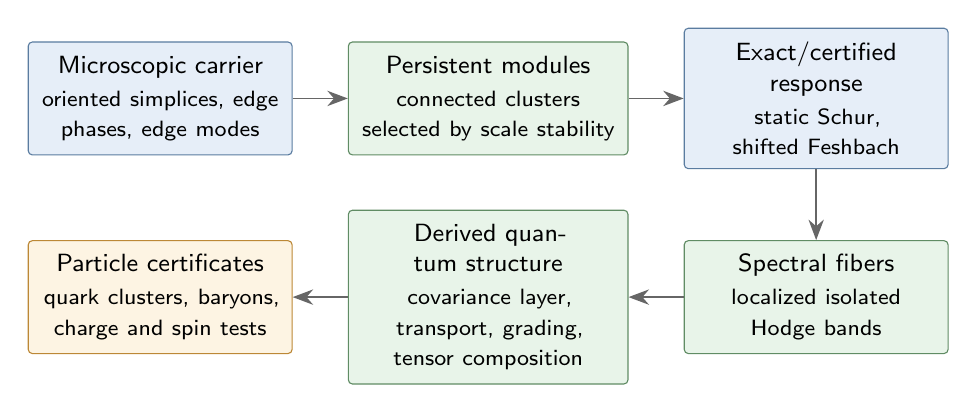
\begin{tikzpicture}[node distance=6mm and 7mm]
  \node[estbox,text width=30mm] (carrier) {Microscopic carrier\\[1pt]\footnotesize oriented simplices, edge phases, edge modes};
  \node[derivbox,text width=32mm,right=of carrier] (modules) {Persistent modules\\[1pt]\footnotesize connected clusters selected by scale stability};
  \node[estbox,text width=30mm,right=of modules] (response) {Exact/certified response\\[1pt]\footnotesize static Schur, shifted Feshbach};
  \node[derivbox,text width=30mm,below=9mm of response] (fibers) {Spectral fibers\\[1pt]\footnotesize localized isolated Hodge bands};
  \node[derivbox,text width=32mm,left=of fibers] (derived) {Derived quantum structure\\[1pt]\footnotesize covariance layer, transport, grading, tensor composition};
  \node[propbox,text width=30mm,left=of derived] (certs) {Particle certificates\\[1pt]\footnotesize quark clusters, baryons, charge and spin tests};
  \draw[flow] (carrier) -- (modules);
  \draw[flow] (modules) -- (response);
  \draw[flow] (response) -- (fibers);
  \draw[flow] (fibers) -- (derived);
  \draw[flow] (derived) -- (certs);
\end{tikzpicture}
\caption{Concept map for the recursive complex construction. Colors encode
epistemic status, not physical sectors: blue is established or exact machinery,
green is a derived observable, and amber is a proposed physical
identification.}
\label{fig:concept}
\end{figure}

% ================================================================ 2
\section{Present evidence in Tessera}\label{sec:evidence}

Two existing results motivate the construction.

First, the state-operation-cobordism experiments show that the Hodge-carried
register is a scaled isometry to machine precision --- its Gram is the
identity once one global scale is fixed by the anchor --- and that its spectral
value
reproduces the quantum transition amplitude for every operation that the tested
geometry actually carries. Generic fixed-complexity operations can remain
obstructed, and the obstruction is visible both as a residual floor and as
leakage from the carried subspace. The claim is therefore not that every finite
complex realizes every gate; it is that a realized, isometrically embedded
register computes the corresponding amplitude. See
\code{cobordism-results.md}.

Second, interaction-history complexes exhibit a stable near-four-dimensional
spectral regime. The strongest reported measurements approach, but do not yet
prove, an exact spectral dimension of four. The current status and finite-size
caveats are recorded in \code{h\_ds4\_status.md}. Diffusion-based spectral
dimension on simplicial quantum geometries has important precedent in causal
dynamical triangulations \cite{ajl2005}; the Tessera evidence is an independent
result for a different construction and should be compared at the level of the
return-probability estimator and its finite-size window.

The current proton animation adds a third, more preliminary observation. It
starts with the phase pattern $\{1,\omega,\omega^{2}\}$ and evaluates its
singlet diagnostics while a joint Regge--Hodge stationarity objective changes
the complex. It no longer forces register holes to appear, and holes have not
re-emerged in the current construction. That negative result is useful: the
proposed quark should therefore not be defined as a hole. It will be sought as
a persistent modular spectral cluster, while Betti numbers remain independent
topological observables.

% ================================================================ 3
\section{The microscopic geometric state}\label{sec:state}

Let \code{K} be a finite oriented simplicial complex. For every edge $e$, store
the complex squared length
\begin{equation*}
  z_{e}=\rho_{e}e^{i\theta_{e}}\in\mathbb{C}
\end{equation*}
and, separately, the connection phase
\begin{equation*}
  \varphi_{e}\in\mathbb{C},
\end{equation*}
and attach the two-level occupation factor
$\HK_{e}=\operatorname{span}\{\lvert 0\rangle_{e},\lvert 1\rangle_{e}\}$.

The two edge fields are distinct, and the reason is gauge invariance. The
connection transforms as $\varphi\mapsto\varphi+d\chi$ while the geometry must
not: were $\varphi_{e}$ taken to be $\arg z_{e}$, a gauge transformation would
change the squared length --- that is, it would change the metric. So the phase
is carried as its own field and enters the metric weight multiplicatively,
\begin{equation*}
  w_{e}=z_{e}\,e^{i\varphi_{e}},
\end{equation*}
the discrete magnetic coupling: geometry times a link phase. Saying that an edge
``carries a qubit'' means that it carries the local mode algebra above, not that
the global state is forced to be a product of normalized vectors $q_{e}$.

Because $\varphi_{e}$ is complex,
$e^{i\varphi}=e^{i\operatorname{Re}\varphi}e^{-\operatorname{Im}\varphi}$, and
the structure group is $\mathbb{C}^{*}=U(1)\times\mathbb{R}^{+}$: a compact part
and a non-compact one. Only the compact part has winding, so only the compact
part quantizes; the non-compact part acts as a local scale and carries no
quantum number. Four consequences follow and are used throughout:
\begin{itemize}
  \item $L$ is generically \emph{non-normal}, not merely Krein-indefinite, so
    matched left and right frames with $\Psi^{\dagger}W\Phi=I$ are mandatory
    rather than a fallback;
  \item eigenvalues are properly complex, so band isolation must be measured as
    separation in the complex plane and never to a sort-order neighbour;
  \item band projectors are oblique, so $\Gamma=P$ is the covariance of an actual
    state only where the restricted metric is definite --- a Krein-definite band
    --- while an indefinite band admits no state at all; and
  \item under a similarity $L\mapsto SLS^{-1}$ eigenvalues are invariant while
    eigenvectors are only covariant, so observables must be spectral or
    holonomy-valued. This strengthens rather than weakens the discipline the rest
    of the paper already imposes on Wilson loops and the determinant line.
\end{itemize}

The edge data are not the state. They parameterize the operator; the state is
the spectral data of $L(z,\varphi)$ --- its eigenvalues and its selected
eigenspaces, entering below as band projectors. An edge datum is a coordinate on
the space of operators, not an amplitude.

Writing $\hh_{K}=\operatorname{span}\{\lvert e\rangle : e\in K_{1}\}$ for the
one-particle edge space, the microscopic quantum carrier is
\begin{equation*}
  \HK_{K}=\Fock(\hh_{K})=\Lambda^{\bullet}\hh_{K}
  \;\cong\;\widehat{\bigotimes}_{e\in K_{1}}\HK_{e},
\end{equation*}
and a boundary state is a vector or density operator on $\HK_{K}$. It may be
entangled. A one-particle color state $a^{\dagger}_{\phi}\lvert 0\rangle$ and
the nonseparable proton-spin sectors are therefore native states, not
exceptions to the ontology. For an isolated occupied band with projector $P$,
the corresponding quasi-free reference state has covariance
\begin{equation*}
  \Gamma_{ef}=\langle a^{\dagger}_{f}a_{e}\rangle=P_{ef},
  \qquad \langle n_{e}\rangle=P_{ee}.
\end{equation*}
Thus a per-edge Bloch vector or occupation is a derived marginal/readout. The
quasi-free state is a useful analytic baseline, not a restriction of the state
space: the lazy Fock construction of Section~\ref{sec:fock} can represent
explicitly non-Gaussian sectors. Section~\ref{sec:quasifree} records, however,
that no generator currently present in the model produces such sectors from
Gaussian data; until one of the mechanisms listed there is adopted,
non-Gaussianity can enter only as boundary data.

Let
\begin{equation*}
  \partial_{k}:C_{k}(K)\longrightarrow C_{k-1}(K),
  \qquad \partial_{k-1}\partial_{k}=0
\end{equation*}
be the oriented boundary maps and let \code{W\_k(z)} be the metric weight on
\code{k}-chains. With the weighted adjoint
\begin{equation*}
  \partial^{*}_{k}=W_{k}^{-1}\partial^{\dagger}_{k}W_{k-1},
\end{equation*}
the degree-\code{k} Hodge Laplacian is
\begin{equation*}
  L_{k}=\partial_{k+1}\partial^{*}_{k+1}+\partial^{*}_{k}\partial_{k}.
\end{equation*}
In the positive metric regime this is self-adjoint in the \code{W\_k} inner
product. In the signed Lorentzian regime it can be non-normal; then left and
right spectral frames and their biorthogonal condition numbers must be reported
rather than silently treating \code{L\_k} as Hermitian.

The geometry evolves toward joint stationary points of the existing Regge and
Hodge functionals. In emergence mode, particle-specific observables below are
read after optimization and are not inserted as target terms. Controlled
synthesis mode may pin a carrier to test realizability, but that is a separate
experiment. Section~\ref{sec:quasifree} refines the emergence protocol into two
labeled modes --- strict no-backreaction, and certificates-blind mean-field
backreaction --- and records that both remain inside the quasi-free class.

This operator stack sits on established foundations: Regge calculus encodes
piecewise-flat gravity in simplicial deficit angles \cite{regge1961}, discrete
exterior calculus supplies metric-dependent chain/cochain operators
\cite{dec2005}, and combinatorial Hodge spectra on simplicial complexes have a
developed spectral theory \cite{horakjost2013}. Tessera's proposal is not a
replacement for those constructions; it is a constrained use of them as the
sole source of the later particle readouts.

% ================================================================ 4
\section{A component is an exact static response vertex}\label{sec:vertex}

Partition the \code{k}-cells of a connected component into interface cells
\code{B} and interior cells \code{I}, and block its Hodge operator as
\begin{equation*}
  L=\begin{pmatrix} L_{BB} & L_{BI}\\ L_{IB} & L_{II}\end{pmatrix}.
\end{equation*}
In the positive self-adjoint regime, after projecting out incompatible interior
zero modes, minimization over the interior has the exact solution
\begin{equation*}
  x_{I}^{*}=-L_{II}^{+}L_{IB}x_{B},
\end{equation*}
and the exact effective boundary operator
\begin{equation*}
  \boxed{\,L_{\mathrm{eff}}=L_{BB}-L_{BI}L_{II}^{+}L_{IB}\,}.
\end{equation*}
Here \code{+} denotes the Moore--Penrose inverse on the supported interior
subspace. For every compatible boundary value,
\begin{equation*}
  \min_{x_{I}}
  \begin{pmatrix}x_{B}\\ x_{I}\end{pmatrix}^{\dagger}
  L
  \begin{pmatrix}x_{B}\\ x_{I}\end{pmatrix}
  = x_{B}^{\dagger}L_{\mathrm{eff}}x_{B}.
\end{equation*}

This is the precise static, or zero-frequency, sense in which a connected
component can be replaced by a coarse response vertex. In a Hermitian
indefinite regime the same equation is a stationarity condition, not a minimum.
For a non-normal block it is simply block elimination; solvability requires
\begin{equation*}
  L_{IB}x_{B}\perp\ker L_{II}^{\dagger}.
\end{equation*}

The plain Schur complement does \emph{not} preserve the nonzero spectrum. For a
spectral parameter $\lambda$ such that $L_{II}-\lambda I$ is invertible, define
the exact Feshbach--Schur response
\begin{equation*}
  \boxed{\,F_{B}(\lambda)=L_{BB}-\lambda I
    - L_{BI}(L_{II}-\lambda I)^{-1}L_{IB}\,}.
\end{equation*}
Then, for $\lambda$ outside $\operatorname{spec}L_{II}$, the exact determinant
factorization
\begin{equation*}
  \det(L-\lambda I)=\det(L_{II}-\lambda I)\,\det F_{B}(\lambda)
\end{equation*}
holds, so
\begin{equation*}
  \lambda\in\operatorname{spec}L \iff 0\in\operatorname{spec}F_{B}(\lambda).
\end{equation*}
The order of the zero of $\det F_{B}(\cdot)$ at $\lambda$ equals the algebraic
multiplicity of $\lambda$ in $L$, while $\dim\ker F_{B}(\lambda)$ equals its
geometric multiplicity; the two agree in the self-adjoint or otherwise
semisimple setting but not in general. At an interior resonance the inverse is
replaced only after checking the compatibility condition
$L_{IB}x_{B}\perp\ker(L_{II}-\lambda I)^{\dagger}$ and retaining the resonant
interior modes explicitly. Thus harmonic response uses $F_{B}(0)$, while a
localized band centered at $\lambda_{C}$ uses $F_{B}(\lambda)$ over a stated
frequency window. A linear reduced eigenproblem may instead retain interface
constraint modes plus selected fixed-interface modes using Craig--Bampton
component-mode synthesis or AMLS; that route is certified approximation whose
error is controlled by residuals and separation from discarded modes, not an
exact spectral identity \cite{craigbampton1968,bennighoflehoucq2004,bcfs2003}.

The effective blocks between coarse components become operator-valued links. A
harmonic or retained interior mode is not discarded; it becomes an explicit
stalk/fiber coordinate attached to the response vertex.

For graph Laplacians this is the classical Kron reduction by Schur complement
\cite{dorflerbullo2013}. Spectral graph reduction provides related
approximation guarantees when additional coarsening or truncation is performed
\cite{loukas2019}. The extension proposed here is to apply static response
reduction degree by degree to weighted Hodge blocks, and shifted Feshbach or
certified component-mode reduction to nonzero bands, while retaining localized
zero, resonant, and selected interior modes as explicit fiber coordinates.

% ================================================================ 5
\section{Recursive spectral fibers}\label{sec:fibers}

Let $P_{\ell}=\{C_{v}^{\ell}\}$ be an intrinsic partition at scale $\ell$ into
persistent connected components. At $\ell=0$ the object is the microscopic
simplicial complex $K_{0}$. After the first elimination the honest coarse
object is generally not another simplicial complex: it is an operator-valued
response network $\RN_{\ell+1}$ whose vertices carry vector spaces and whose
links carry linear response blocks. A cellular sheaf on the quotient graph is a
natural realization when the blocks admit compatible restriction-map
factorization \cite{hansenghrist2019}; otherwise Tessera retains the more
general response network and does not invent incidence maps that the reduction
did not determine.

Within component \code{C}, choose an isolated localized spectral band and, in
the positive self-adjoint regime, a weighted orthonormal frame
\begin{equation*}
  \Phi_{C}=(\phi_{1},\dots,\phi_{r}),
  \qquad \Phi_{C}^{\dagger}W_{C}\Phi_{C}=I_{r}.
\end{equation*}
The derived fiber is
\begin{equation*}
  E_{C}=\operatorname{Ran}\Phi_{C}.
\end{equation*}

In a Hermitian indefinite regime record the inertia of
$\Phi_{C}^{\dagger}W_{C}\Phi_{C}$ and normalize it to a signature matrix
$J_{C}=\operatorname{diag}(I_{p},-I_{q})$. Negative Krein signature is a
certificate, not an automatic identification with an antiparticle. Existing
Tessera pair-creation experiments do, however, exhibit an opposite-signature
selection rule with conserved real part under conjugate-pair formation; that
measured behavior is second-tier evidence for the particle/antiparticle
reading, while the identification itself remains a third-tier proposed
interpretation. In a non-normal regime use matched right and left frames
$\Phi_{C},\Psi_{C}$ with $\Psi_{C}^{\dagger}W_{C}\Phi_{C}=I$ and report both
residuals and the frame condition number.

It need not be a harmonic space and therefore need not be supported by a hole.
What it does require is a spectral gap, localization, and persistence. A
candidate component is accepted only if all of the following remain stable
across a stated range of scales:
\begin{itemize}
  \item a persistent connected cluster support, however proposed;
  \item a localized spectral projector with stable rank;
  \item a nonzero band gap separating it from discarded modes;
  \item overlap with its predecessor and successor components;
  \item lifetime across multiple cobordism frames; and
  \item small external transport leakage.
\end{itemize}

Community objectives supply deterministic cluster candidates
\cite{reichardtbornholdt2006}, while network renormalization supplies tests for
genuine self-similarity rather than visual resemblance \cite{songhavlin2005}.
The partition is therefore a measured part of the analysis: a recursively drawn
pattern is not evidence of a fractal unless its scaling observables survive a
refinement window. The current \code{ModularityOptimizer} uses Newman--Girvan
modularity on a combinatorial one-skeleton; it is a heuristic proposal
generator that does not see signed or complex Hodge weights and is subject to
the modularity resolution limit \cite{fortunatobarthelemy2007}. Modularity may
therefore propose candidate supports, but it may not veto an otherwise
certified fiber: acceptance is conditioned only on the independent,
weight-aware gap, localization, leakage, persistence, and refinement
certificates above, together with the anchoring certificate of
Section~\ref{sec:quarks} whenever a color interpretation is claimed.

This gives a type-stable hierarchy of response objects
\begin{equation*}
  \cdots\longrightarrow\RN_{2}\longrightarrow\RN_{1}\longrightarrow K_{0}
\end{equation*}
in which a response vertex at one level resolves into a connected microscopic
component plus retained stalk coordinates at the next finer level.
``Self-similar'' refers to closure of the response-network data type, not to a
claim that every reduced operator is a simplicial Hodge Laplacian. A
fractal-like pattern is permitted but not required: measured scaling of module
count, volume, boundary size, and spectral gap decides whether the hierarchy is
statistically self-similar.

\begin{figure}[htb]
\centering
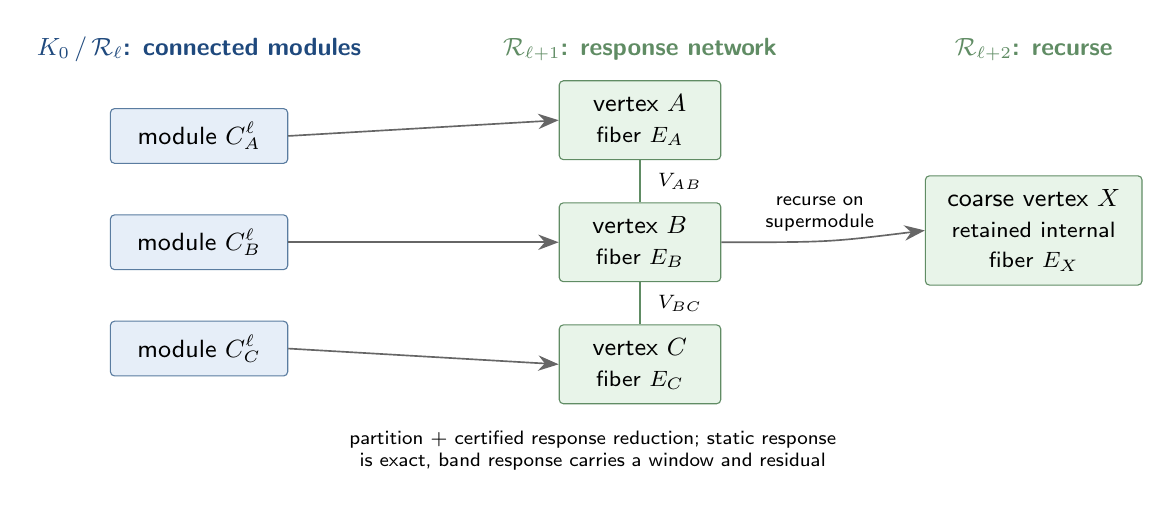
\begin{tikzpicture}
  % column headers
  \node[font=\small\sffamily\bfseries\color{headblue}] at (0,2.45) {$K_{0}\,/\,\RN_{\ell}$: connected modules};
  \node[font=\small\sffamily\bfseries\color{derivgreenline}] at (5.6,2.45) {$\RN_{\ell+1}$: response network};
  \node[font=\small\sffamily\bfseries\color{derivgreenline}] at (10.6,2.45) {$\RN_{\ell+2}$: recurse};
  % left: microscopic modules
  \node[estbox,text width=19mm] (mA) at (0,1.35) {module $C_{A}^{\ell}$};
  \node[estbox,text width=19mm] (mB) at (0,0)    {module $C_{B}^{\ell}$};
  \node[estbox,text width=19mm] (mC) at (0,-1.35){module $C_{C}^{\ell}$};
  % middle: response network
  \node[derivbox,text width=17mm] (vA) at (5.6,1.55) {vertex $A$\\ \footnotesize fiber $E_{A}$};
  \node[derivbox,text width=17mm] (vB) at (5.6,0)    {vertex $B$\\ \footnotesize fiber $E_{B}$};
  \node[derivbox,text width=17mm] (vC) at (5.6,-1.55){vertex $C$\\ \footnotesize fiber $E_{C}$};
  \draw[semithick,draw=derivgreenline] (vA) -- (vB)
    node[midway,right=1mm,font=\scriptsize\sffamily]{$V_{AB}$};
  \draw[semithick,draw=derivgreenline] (vB) -- (vC)
    node[midway,right=1mm,font=\scriptsize\sffamily]{$V_{BC}$};
  % right: recursion
  \node[derivbox,text width=24mm] (X) at (10.6,0.15)
    {coarse vertex $X$\\ \footnotesize retained internal fiber $E_{X}$};
  % arrows
  \draw[flow] (mA.east) -- (vA.west);
  \draw[flow] (mB.east) -- (vB.west);
  \draw[flow] (mC.east) -- (vC.west);
  \draw[flow] (vB.east) .. controls (8.0,0) .. (X.west)
    node[pos=0.45,above,font=\scriptsize\sffamily,align=center]{recurse on\\supermodule};
  \node[font=\scriptsize\sffamily,align=center,text width=105mm] at (5.0,-2.65)
    {partition $+$ certified response reduction; static response is exact, band response carries a window and residual};
\end{tikzpicture}
\caption{One recursive step. Persistent connected modules become stalk-bearing
vertices of an operator-valued response network. Static response is preserved
by the supported Schur complement; nonzero bands use shifted Feshbach or
certified component-mode reduction. Selected internal modes remain attached as
fibers, and a persistent supermodule can be reduced again at the next scale.}
\label{fig:recursion}
\end{figure}

% ================================================================ 6
\section{Interactions and the expanding Hilbert space}\label{sec:interactions}

Two operations must not be conflated. For the Cartesian product of chain
complexes \code{A} and \code{B}, the graded tensor differential is the exact
rule
\begin{equation*}
  d_{A\gtens B}(a\otimes b)=d_{A}a\otimes b+(-1)^{\deg a}a\otimes d_{B}b.
\end{equation*}
For a noninteracting product with product metric,
\begin{equation*}
  L_{A\gtens B}=L_{A}\otimes I+I\otimes L_{B},
\end{equation*}
so one-particle eigenvalues add and eigenvectors tensor. This identity is about
a product complex, not about gluing two cobordisms.

Actual simplicial gluing is a pushout along a shared boundary. At the
one-particle level it produces a chain space assembled from direct sums modulo
boundary identifications (equivalently described by the relevant
Mayer--Vietoris sequence) and a block operator
\begin{equation*}
  L_{A\cup B}=\begin{pmatrix} L_{A} & C_{AB}\\ C_{BA} & L_{B}\end{pmatrix}
\end{equation*}
in a basis adapted to the two interiors. The coupling blocks are induced by the
connecting simplices and shared-boundary constraints; they are not a Kronecker
interaction term.

The expanding Hilbert space follows after applying the fermionic Fock functor
to the one-particle space $\hh$. The exact identities are
\begin{equation*}
  \Fock(\hh_{A}\oplus\hh_{B})\cong\Fock(\hh_{A})\gtens\Fock(\hh_{B}),
\end{equation*}
and
\begin{equation*}
  \dG(L_{A}\oplus L_{B})=\dG(L_{A})\gtens I+I\gtens\dG(L_{B}).
\end{equation*}
For the coupling block,
\begin{equation*}
  \dG(C_{AB}+C_{BA})
  =\sum_{ij}(C_{AB})_{ij}\,a^{\dagger}_{A,i}a_{B,j}+\text{h.c.},
\end{equation*}
so geometric connections become hopping terms without adding a new field. If
the one-particle eigenvalues are $\lambda_{1},\dots,\lambda_{M}$, then the free
many-body spectrum is the set of occupation subset sums
$\sum_{i}n_{i}\lambda_{i}$, $n_{i}\in\{0,1\}$, rather than the one-particle
pairwise spectrum being relabeled as a Fock spectrum \cite{berezin1966}.

At the selected-fiber level, an interaction grows the carried space as
\begin{equation*}
  \HK_{AB}=E_{A}\gtens E_{B},
\end{equation*}
and a later interaction appends another factor. This is a statement about
state-space composition after second quantization, not the topology of the
glued chain complex. When carried subspaces of adjacent components overlap on
interface cells, the composite is built on the abstract labeled sum with an
explicit embedding Gram matrix; Section~\ref{sec:master} states the exact rule.
If $J_{C}$ embeds an abstract state into the geometric carrier, exact amplitude
preservation requires
\begin{equation*}
  J_{C}^{\dagger}W_{C}J_{C}=I.
\end{equation*}
Tensor products preserve isometry exactly. If $G=J_{C}^{\dagger}W_{C}J_{C}$ has
Gram defect $\varepsilon=\lVert G-I\rVert$, then
\begin{equation*}
  \lvert a^{\dagger}Gb-a^{\dagger}b\rvert
  \le\varepsilon\,\lVert a\rVert\,\lVert b\rVert,
\end{equation*}
and two tensor factors obey
\begin{equation*}
  \varepsilon_{AB}\le\varepsilon_{A}+\varepsilon_{B}
    +\varepsilon_{A}\varepsilon_{B}.
\end{equation*}
Thus the amplitude claim has an explicit, composable error budget.

Cobordism composition as a map between boundary state spaces is the organizing
idea of topological field theory \cite{atiyah1988}; the general-boundary
program makes the region/boundary assignment explicit for quantum theory
\cite{oeckl2003}, and categorical quantum mechanics formalizes tensor
composition and diagrammatic process semantics \cite{abramskycoecke2004}.
Tessera keeps only the parts that can be realized by its finite simplicial
carrier and tests the resulting map numerically rather than assuming
topological invariance.

% ================================================================ 7 (NEW)
\section{Quasi-free dynamics and the covariance layer}\label{sec:quasifree}

Every many-body generator exhibited in this paper is quadratic. Free
propagation is $\dG(L)$, gluing contributes $\dG$ of a coupling block, and
every derived transport is the second quantization of a one-particle map. The
exact consequence is closure of the quasi-free class: if the Hamiltonian is
always of the form
\begin{equation*}
  H(t)=\dG\bigl(h(t)\bigr)=\sum_{ij}h_{ij}(t)\,a^{\dagger}_{i}a_{j},
\end{equation*}
then Gaussian/quasi-free states remain Gaussian.

The closure survives self-consistency. Let the one-particle operator depend on
the covariance and on the classical geometry,
\begin{equation*}
  h=h\bigl(\Gamma(t),g(t)\bigr),
\end{equation*}
with the geometry in turn relaxed against the state's energy density. That is
nonlinear mean-field dynamics of generalized Hartree--Fock type
\cite{bls1994}; it can localize and it can produce self-bound solutions, but it
does not leave the Gaussian manifold. Classical or mean-field geometry
backreaction alone therefore does not generate genuinely non-Gaussian
correlations.

The emergence protocol accordingly splits into two labeled modes, both
Gaussian-closed: \emph{strict emergence}, in which the state does not act back
on the geometry at all, and \emph{certificates-blind mean-field backreaction},
in which the carried state's energy density enters the joint stationarity
objective while every particle certificate remains firewalled from it. The
certificate firewall of Section~\ref{sec:proton} applies to both modes.

Genuinely non-Gaussian correlations would require at least one of the
following, none of which is currently part of the model:
\begin{enumerate}
  \item a genuine quartic effective interaction,
    \begin{equation*}
      H_{\mathrm{int}}
      =\sum_{ijkl}V_{ijkl}\,
        a^{\dagger}_{i}a^{\dagger}_{j}a_{k}a_{l};
    \end{equation*}
  \item quantized geometry that becomes entangled with the fermions;
  \item integrating out dynamical geometry beyond the mean-field
    approximation, producing a retarded or quartic effective interaction;
  \item a cobordism map that is not the second quantization of a one-particle
    map; or
  \item measurement or postselection capable of taking Gaussian states outside
    the Gaussian class.
\end{enumerate}
Adopting one of these is an explicit scope decision with its own certificates,
not a background assumption. Until then, the statement that non-Gaussian
sectors are representable (Section~\ref{sec:state}) must not be read as a
statement that they are produced.

The quasi-free formulation is extremely attractive on its own terms. In the
number-conserving case the entire state is the covariance matrix
\begin{equation*}
  \Gamma_{ij}=\langle a^{\dagger}_{j}a_{i}\rangle,
  \qquad i\dot{\Gamma}=[h,\Gamma],
\end{equation*}
with $\Gamma^{2}=\Gamma$ exactly for a pure Slater state; a pairing sector
would extend $\Gamma$ to the full Nambu covariance without changing the closure
statement. Wick's theorem then computes every polynomial observable exactly:
occupations and parities, the Pauli/Gram determinants, the color wedge
$\lvert S_{ABC}\rvert^{2}$, and both $\langle J^{2}\rangle$ and its variance.
There is no reason to construct an exponential Fock vector except for oracle
tests or for explicitly non-Gaussian boundary data.

The programme order follows. First test the strongest possible covariance-only
theory. Treat failure of the sharp proton certificate of
Section~\ref{sec:proton} as a meaningful structural result rather than a
numerical nuisance. Introduce a non-Gaussian interaction only if the geometry
supplies one naturally, through one of the mechanisms above. The question that
decides the next stage of the programme is stated exactly:

\begin{center}
\fbox{\parbox{0.9\linewidth}{\centering\itshape
Is an exact covariance-only proton possible, or is a genuinely non-Gaussian,
geometry-mediated interaction required?}}
\end{center}

Either answer is informative. A covariance-only proton would make the entire
particle layer polynomially computable and exactly certifiable; a demonstrated
obstruction would be the first internal evidence that the geometry must supply
a true interaction term.

% ================================================================ 8
\section{A triangle carries the exact color algebra}\label{sec:triangle}

Consider the three edge-mode factors around an oriented triangle and interpret
\code{|1>} as an occupied edge mode. Choosing an oriented ordering
$(e_{1},e_{2},e_{3})$ identifies their graded tensor product with the exterior
algebra
\begin{equation*}
  (\mathbb{C}^{2})^{\gtens 3}\cong\Lambda^{\bullet}\mathbb{C}^{3}
  =\mathbf{1}\oplus\mathbf{3}\oplus\overline{\mathbf{3}}\oplus\mathbf{1}.
\end{equation*}
The orientation of one triangle fixes the ordering up to a cyclic, hence even,
permutation, so the local wedge sign is unambiguous. Globally the exterior
algebra $\Lambda^{\bullet}\hh_{K}$ and the CAR are intrinsic; only a
compilation into tensor-product qubits or bitsets needs a deterministic mode
order and the corresponding permutation parity. A Kasteleyn orientation is
useful for two-dimensional surface-dimer Pfaffians but is not required to
define this abstract Fock space \cite{cimasonireshetikhin2007}. A genuine
continuum spinor interpretation is a separate question addressed by the
rotation certificate below.

The sectors have occupation number $N=0,1,2,3$:

\begin{table}[htb]
\centering
\begin{tabular}{lclc}
\toprule
Sector & Basis dimension & Color interpretation & Fermion parity\\
\midrule
$\Lambda^{0}\mathbb{C}^{3}$ & 1 & vacuum & even\\
$\Lambda^{1}\mathbb{C}^{3}$ & 3 & fundamental color triplet & odd\\
$\Lambda^{2}\mathbb{C}^{3}$ & 3 & antisymmetric anti-triplet & even\\
$\Lambda^{3}\mathbb{C}^{3}$ & 1 & color singlet & odd\\
\bottomrule
\end{tabular}
\caption{Exterior sectors of three oriented edge modes.}
\label{tab:sectors}
\end{table}

Let $a^{\dagger}_{i},a_{i}$ be the exterior creation and contraction operators.
They satisfy the canonical anticommutation relations exactly:
\begin{equation*}
  \{a_{i},a_{j}\}=0,\qquad
  \{a^{\dagger}_{i},a^{\dagger}_{j}\}=0,\qquad
  \{a_{i},a^{\dagger}_{j}\}=\delta_{ij}.
\end{equation*}
On the one-occupation sector, the bilinears
\begin{equation*}
  E_{ij}=a^{\dagger}_{i}a_{j}
\end{equation*}
satisfy
\begin{equation*}
  [E_{ij},E_{k\ell}]=\delta_{jk}E_{i\ell}-\delta_{i\ell}E_{kj}.
\end{equation*}
The six Hermitian off-diagonal combinations together with
\begin{equation*}
  H_{1}=E_{11}-E_{22},\qquad
  H_{2}=\frac{E_{11}+E_{22}-2E_{33}}{\sqrt{3}}
\end{equation*}
are the eight generators of $\su(3)$. Thus the triangle does not merely hold
three phases: its one-particle edge sector carries the fundamental
representation, its two-particle sector carries the dual representation, and
its traceless bilinears carry the adjoint octet.

The triplet description of quarks and the three-quark construction of baryons
originate with the quark model \cite{gellmann1964}; the additional color
triplet was introduced to resolve the statistics and state-counting problem
\cite{hannambu1965,greenberg1964}. The claim here is narrower and new:
Tessera's three oriented edge modes would provide a geometric carrier of the
same representation content, not a derivation of QCD from the combinatorics
alone.

\begin{figure}[htb]
\centering
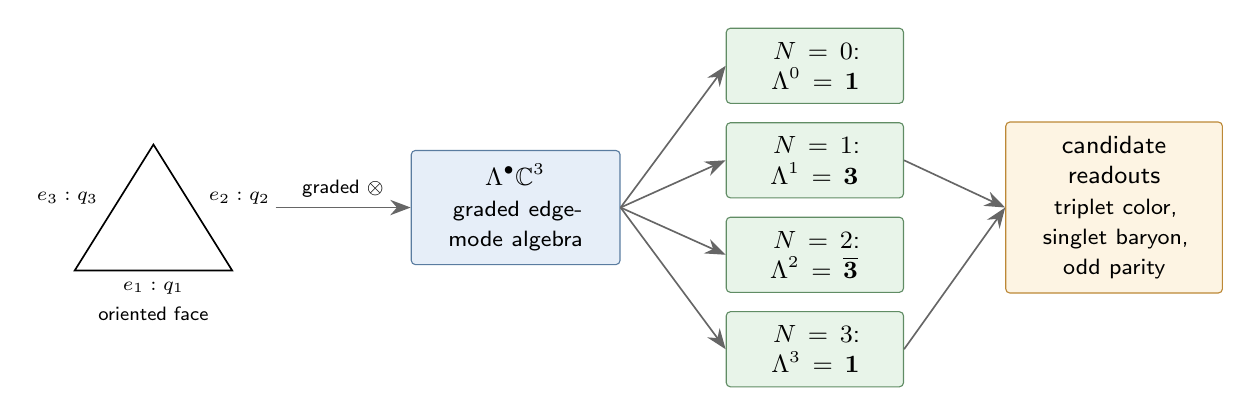
\begin{tikzpicture}
  % triangle
  \coordinate (t1) at (0,0);
  \coordinate (t2) at (2.0,0);
  \coordinate (t3) at (1.0,1.6);
  \draw[semithick] (t1)--(t2)--(t3)--cycle;
  \node[font=\scriptsize\sffamily,below] at (1.0,-0.02) {$e_{1}:q_{1}$};
  \node[font=\scriptsize\sffamily,right] at (1.58,0.92) {$e_{2}:q_{2}$};
  \node[font=\scriptsize\sffamily,left] at (0.42,0.92) {$e_{3}:q_{3}$};
  \node[font=\scriptsize\sffamily] at (1.0,-0.55) {oriented face};
  % algebra box
  \node[estbox,text width=23mm] (alg) at (5.6,0.8) {$\Lambda^{\bullet}\mathbb{C}^{3}$\\ \footnotesize graded edge-mode algebra};
  \draw[flow] (2.55,0.8) -- (alg.west)
    node[pos=0.5,above,font=\scriptsize\sffamily]{graded $\otimes$};
  % sectors
  \node[derivbox,text width=19mm] (n1) at (9.4,2.6)  {$N=0$: $\Lambda^{0}=\mathbf{1}$};
  \node[derivbox,text width=19mm] (n2) at (9.4,1.4)  {$N=1$: $\Lambda^{1}=\mathbf{3}$};
  \node[derivbox,text width=19mm] (n3) at (9.4,0.2)  {$N=2$: $\Lambda^{2}=\overline{\mathbf{3}}$};
  \node[derivbox,text width=19mm] (n4) at (9.4,-1.0) {$N=3$: $\Lambda^{3}=\mathbf{1}$};
  \draw[flow] (alg.east) -- (n1.west);
  \draw[flow] (alg.east) -- (n2.west);
  \draw[flow] (alg.east) -- (n3.west);
  \draw[flow] (alg.east) -- (n4.west);
  % readouts
  \node[propbox,text width=24mm] (read) at (13.2,0.8) {candidate readouts\\ \footnotesize triplet color, singlet baryon, odd parity};
  \draw[flow] (n2.east) -- (read.west);
  \draw[flow] (n4.east) -- (read.west);
\end{tikzpicture}
\caption{Exact representation content of three oriented edge-mode factors. The
exterior sectors and their parity are algebraic identities. Interpreting the
rank-three odd sector as quark color and the top wedge as a baryon color
singlet is the physical hypothesis to be tested.}
\label{fig:triangle}
\end{figure}

\subsection{Geometric normalization}

For the stored complex squared lengths $z_{i}=\rho_{i}e^{i\theta_{i}}$ on the
three oriented edges, define
\begin{equation*}
  c_{i}=\frac{z_{i}}
    {\sqrt{\lvert z_{1}\rvert^{2}+\lvert z_{2}\rvert^{2}
      +\lvert z_{3}\rvert^{2}}},
  \qquad
  \lvert c\rangle=\sum_{i=1}^{3}c_{i}\lvert i\rangle.
\end{equation*}
Then $\langle c|c\rangle=1$. Constraining the perimeter to one is a valid
geometric scale gauge, but it is an \code{L\^{}1} condition and does not
replace the $L^{2}$ Hilbert normalization. Normalized pure color states form
$\mathbb{CP}^{2}$; $SU(3)$ is the transformation group, not the surface of the
triangle itself.

\subsection{The existing omega phase pattern}

Let $\omega=e^{2\pi i/3}$. The exact Fourier frame
\begin{equation*}
  F_{3}=\frac{1}{\sqrt{3}}
  \begin{pmatrix}
    1 & 1 & 1\\
    1 & \omega & \omega^{2}\\
    1 & \omega^{2} & \omega
  \end{pmatrix}
\end{equation*}
is unitary. The existing pattern $(1,\omega,\omega^{2})/\sqrt{3}$ is therefore
one color basis vector, not by itself the whole color fiber. Its cyclic orbit
supplies an exact orthonormal triad.

% ================================================================ 9
\section{Color transport and Wilson loops without a new gauge field}
\label{sec:transport}

Let $T_{AB}$ be the chain-level transfer already induced by connecting
simplices from component $B$ to component $A$. In positive self-adjoint local
spectral frames of common rank $r$, the raw fiber map is
\begin{equation*}
  M_{AB}=\Phi_{A}^{\dagger}W_{A}T_{AB}\Phi_{B}.
\end{equation*}
Its departure from an isometry is a physical leakage diagnostic:
\begin{equation*}
  \eta_{AB}=\lVert M_{AB}^{\dagger}M_{AB}-I\rVert.
\end{equation*}
When the selected band is isolated, $M_{AB}$ has full numerical rank, and
$\eta_{AB}$ is small, take the polar unitary
\begin{equation*}
  V_{AB}=M_{AB}(M_{AB}^{\dagger}M_{AB})^{-1/2}\in U(r).
\end{equation*}
Under a change of local spectral frame, $\Phi_{A}\mapsto\Phi_{A}g_{A}$ and
$\Phi_{B}\mapsto\Phi_{B}g_{B}$,
\begin{equation*}
  V_{AB}\longmapsto g_{A}^{\dagger}V_{AB}g_{B}.
\end{equation*}
Consequently the full closed holonomy and its normalized trace transform by
conjugation at the base point:
\begin{equation*}
  H(\gamma)=\prod_{(AB)\in\gamma}V_{AB},
  \qquad
  W_{U(r)}(\gamma)=\frac{1}{r}\operatorname{Tr}H(\gamma).
\end{equation*}

At rank three there is no globally single-valued operation
$V\mapsto V/(\det V)^{1/3}$: the cube root is $\mathbb{Z}_{3}$-ambiguous. The
faithful derived datum is therefore retained as
\begin{equation*}
  V_{AB}\in U(3),\qquad
  \delta_{AB}=\det V_{AB}\in U(1),\qquad
  [V_{AB}]\in PU(3)\cong SU(3)/\mathbb{Z}_{3}.
\end{equation*}
A local $SU(3)$ lift $\widetilde{U}_{AB}=\delta_{AB}^{-1/3}V_{AB}$ may be
followed continuously along a path after fixing a base branch, but its
accumulated center sector must be reported. Fundamental Wilson traces use the
full $U(3)$ holonomy or an explicitly lifted path; adjoint/projective Wilson
loops are center-blind and require no branch. This turns the former ambiguity
into two measured sectors rather than silently discarding one.

The determinant line also supplies a possible oriented flux readout. For a
closed, full-rank world-tube family $V(t)$,
\begin{equation*}
  \nu=\frac{1}{2\pi}\oint d\,\arg\det V(t)\in\mathbb{Z}
\end{equation*}
is homotopy-invariant while the gap and rank remain open, and changes sign when
the tube orientation is reversed. The integer character of $\nu$ requires the
closed loop. A quark or proton world tube on a cobordism segment is an
interval, and its raw endpoint change of $\arg\det V$ is a phase difference,
not an invariant. The open-segment definition is therefore relative: either
compose the physical transport with the inverse of a matched reference
transport --- the same non-exchanging reference construction used in
Section~\ref{sec:exchange} --- so that the composite closes, or fix endpoint
trivializations supplied by the boundary registers. The reported $\nu$ is the
integer winding of that closed composite, together with its reference
specification. Without such closure $\nu$ is merely an endpoint phase change
and is not certified. Identifying $B=\nu/3$ for an accepted quark tube is a
proposed physical interpretation, not a group identity. Conservation under
pair creation is exact only for a continuous conjugate-pair homotopy with no
determinant zero or boundary flux.

For non-normal bands the correct overlap is biorthogonal,
\begin{equation*}
  M_{AB}=\Psi_{A}^{\dagger}W_{A}T_{AB}\Phi_{B},
  \qquad
  \Psi_{C}^{\dagger}W_{C}\Phi_{C}=I.
\end{equation*}
It is generally a $GL(r,\mathbb{C})$ transport, not a unitary one; left and
right residuals, singular values, and frame condition numbers are part of the
observable. In an indefinite Hermitian sector the Krein inertia is reported and
a pseudo-unitary reduction is attempted only when the two signatures agree. No
$U(r)$ or $SU(3)$ Wilson value is emitted by silently applying the
positive-metric formula outside its domain.

Polar normalization must never conceal a bad fiber assignment: every accepted
holonomy is reported together with $\eta_{AB}$, rank/singular value thresholds,
endpoint band gaps, and frame conditioning.

This construction is the discrete spectral-frame analogue of Berry transport
\cite{berry1984} and its non-Abelian Wilczek--Zee generalization
\cite{wilczekzee1984}. Overlap matrices are also a standard route to
gauge-covariant lattice observables \cite{fukui2005}, as are connection
Laplacians and vector diffusion maps \cite{singerwu2012}. Wilson loops
themselves are foundational lattice gauge observables \cite{wilson1974}. What
is specific here is that the link matrix is not independently assigned: it is
reconstructed from neighboring Hodge frames and accompanied by a leakage
certificate.

% ================================================================ 10
\section{Quarks as modular clusters}\label{sec:quarks}

A \emph{quark candidate} is proposed to be a component \code{Q} satisfying all
of the following derived conditions.

The abstract rank-three band must first be anchored to oriented two-simplices.
For an oriented triangle $\tau\subset Q$, let
$R_{\tau}:C_{1}(Q)\to\mathbb{C}^{3}$ restrict a one-chain to the three ordered
boundary edges, including their incidence signs, and let
$\lvert W_{\tau}\rvert$ be the modulus of the edge-weight block on those three
edges. Define the weighted restriction
\begin{equation*}
  A_{\tau}=\lvert W_{\tau}\rvert^{1/2}R_{\tau}\Phi_{Q}.
\end{equation*}
For a rank-three frame $\Phi_{Q}$, define the gauge-invariant anchor score
\begin{equation*}
  a_{Q}^{2}=\sum_{\tau\subset Q}w_{\tau}\,
    \bigl\lvert\det A_{\tau}\bigr\rvert^{2},
  \qquad w_{\tau}\ge 0,\qquad \sum_{\tau}w_{\tau}=1,
\end{equation*}
with the convex weighting $\{w_{\tau}\}$ declared before the data are examined.
In the positive regime $R_{\tau}^{\dagger}\lvert W_{\tau}\rvert
R_{\tau}\preceq W$, so each
$\lvert\det A_{\tau}\rvert^{2}=\det(A_{\tau}^{\dagger}A_{\tau})\le 1$ and the
score is calibrated: $a_{Q}^{2}\in[0,1]$, with value one exactly at full
concentration on the weighted edge span of the anchoring faces. In signed
sectors the restriction still uses $\lvert W_{\tau}\rvert^{1/2}$ and the Krein
signature of the restricted block is reported separately.

The phases of the nonzero determinants give a local determinant-line
trivialization; their coherence on overlapping triangles is recorded
separately. The reported anchor datum is the profile, not only the score: the
maximal term $\max_{\tau}\lvert\det A_{\tau}\rvert^{2}$, the participation
ratio of the distribution $\{\lvert\det A_{\tau}\rvert^{2}\}$, and the
determinant-phase dispersion accompany $a_{Q}^{2}$. Concentration on one
triangle is a sufficient special case, not a requirement: an extended fiber may
be anchored by an atlas of oriented faces. Because every 2-simplex has exactly
three boundary edges, this anchor is independent of the ambient spectral
dimension.

\begin{enumerate}
  \item \code{Q} is a persistent cluster certified as in
    Section~\ref{sec:fibers}, however its support was proposed.
  \item Its selected color fiber has stable rank three.
  \item Its calibrated triangle-anchor profile and determinant-line coherence
    are stable.
  \item It occupies an odd exterior sector.
  \item Its color transport has bounded leakage over its lifetime.
  \item Its determinant line has an accepted relative winding $\nu=\pm 1$ in
    the closed-composite sense of Section~\ref{sec:transport}; reversing the
    tube yields the dual color representation and an antiquark.
  \item Its total spectral fingerprint is stable under refinement and vertex
    relabeling.
\end{enumerate}

The distinction between an antiquark and the $\Lambda^{2}\mathbb{C}^{3}$
anti-triplet of two quarks is made by determinant-line orientation and total
occupation, not color alone. Assigning $B=\nu/3$ is accepted only when the
winding certificate above exists. A forward/reverse pair then has zero total
winding under a gap-preserving conjugate homotopy; without that certificate
baryon number remains unknown rather than being inserted by definition.

Flavor and electric charge are not assumed as hidden labels. The conservative
hypothesis is that two stable subclasses of the same cluster fiber provide an
isospin doublet. On such a doublet, the measured orientation flux supplies
baryon number and the standard relation
\begin{equation*}
  Q=I_{3}+\frac{B}{2}
\end{equation*}
gives $Q_{u}=+2/3$ and $Q_{d}=-1/3$. This is a proposed identification, not
yet a derivation: it succeeds only if an unlabeled two-dimensional spectral
band emerges, is transported coherently, and its Gauss-flux readout agrees
with those values.

% ================================================================ 11
\section{Fermion statistics from simplicial orientation}\label{sec:statistics}

The graded interchange law is
\begin{equation*}
  \tau(a\gtens b)=(-1)^{F_{a}F_{b}}\,b\gtens a.
\end{equation*}
Two odd clusters therefore acquire a minus sign on exchange, while an even
composite does not. Parity adds modulo two:

\begin{table}[htb]
\centering
\begin{tabular}{lcc}
\toprule
Object & Odd constituents & Composite parity\\
\midrule
quark or antiquark & 1 & odd\\
meson $q\bar{q}$ & 2 & even\\
diquark $qq$ & 2 & even\\
baryon $qqq$ & 3 & odd\\
\bottomrule
\end{tabular}
\caption{Composite exchange parity from constituent counting.}
\label{tab:parity}
\end{table}

Pauli exclusion is the exact exterior-algebra identity
\begin{equation*}
  \lVert v_{1}\wedge\cdots\wedge v_{n}\rVert^{2}
  =\det[\langle v_{i},v_{j}\rangle].
\end{equation*}
If two complete one-particle modes coincide, the determinant and the state
vanish. The ``complete'' qualifier prevents double-counting signs: color, spin,
flavor, space, and component support are wedged once as one mode. One must not
multiply an extra fermion sign by the sign already present in the color epsilon
tensor.

\subsection{A label-independent exchange experiment}\label{sec:exchange}

Let $\Phi_{t}$ be an orthonormal frame for the isolated odd subspace at frame
$t$. Define the parallel transport
\begin{equation*}
  R_{t}=\operatorname{polar}(\Phi_{t+1}^{\dagger}W_{t}\Phi_{t}),
  \qquad
  U_{\gamma}=R_{T-1}\cdots R_{0}.
\end{equation*}
The raw determinant line contains both permutation statistics and an ordinary
Abelian Berry phase:
\begin{equation*}
  \chi_{\mathrm{raw}}(\gamma)=\det U_{\gamma}.
\end{equation*}
It is therefore not expected to equal $\pm 1$ on a generic geometric loop. Let
$\gamma_{0}$ be a non-exchanging reference motion with the same geometric
footprint, timing, and local frame convention. The interferometric exchange
character is
\begin{equation*}
  \widehat{\chi}_{F}(\gamma)=\frac{\det U_{\gamma}}{\det U_{\gamma_{0}}}.
\end{equation*}
The proposed dynamical test is
\begin{equation*}
  \widehat{\chi}_{F}(\text{single exchange})=-1,
  \qquad
  \widehat{\chi}_{F}(\text{double exchange})=+1.
\end{equation*}

As an independent structural cross-check, persistent component matching
extracts the permutation $P_{\gamma}$ of localized odd blocks and reports
$\operatorname{sgn}P_{\gamma}$ together with the norm of the residual in-block
motion after comparison with the reference loop. The algebraic wedge sign is
exact; the interferometric holonomy is the dynamical certificate.

A physical $2\pi$ rotation uses the same reference normalization, and the
rotation path is not left abstract: it is a closed loop constructed here on
the total-space frame, normalized against its own co-moving, non-rotating
reference. It acts on the $J^{2}$ operator whose oracle values are recorded in
\code{joint\_proton\_spin\_findings.md}; that document supplies the operator
and its values, not the cycle, and records the total-space spin readout as an
open item. If an emergent
manifold-like regime supplies tangent frames, a continuum spinor claim
additionally requires a lift of the frame holonomy from $SO(d)$ to
$\mathrm{Spin}(d)$; obstruction by the second Stiefel--Whitney class is then a
falsification certificate \cite{lawsonmichelsohn1989}. This requirement
concerns the physical spin lift, not the existence of the abstract CAR/Fock
algebra. The spin-statistics comparison is cleanest as
\begin{equation*}
  \widehat{\chi}_{F}(\text{exchange})\,
  \widehat{\chi}_{F}(2\pi\ \text{rotation})^{-1}=+1,
\end{equation*}
with each factor separately near $-1$.

Configuration-space topology already explains how exchange classes can carry
quantum phases \cite{laidlawdewitt1971} and, in two dimensions, more general
statistics \cite{leinaasmyrheim1977}. The Tessera proposal uses this precedent
only as a diagnostic template. The minus sign from the graded exterior algebra
is exact; the claim that an actual geometric exchange cobordism realizes the
corresponding determinant holonomy remains an experiment.

% ================================================================ 12
\section{Fock space as an inductive limit of interactions}\label{sec:fock}

For $M$ oriented fermionic edge modes,
\begin{equation*}
  \widehat{\bigotimes}_{m=1}^{M}\mathbb{C}^{2}
  \cong\Lambda^{\bullet}\mathbb{C}^{M}
  =\bigoplus_{n=0}^{M}\Lambda^{n}\mathbb{C}^{M},
\end{equation*}
and the dimension identity is exact:
\begin{equation*}
  2^{M}=\sum_{n=0}^{M}\binom{M}{n}.
\end{equation*}

The exterior algebra is canonical as a functor of the one-particle space.
Writing it as a literal ordered qubit tensor product, or implementing creation
operators by Jordan--Wigner/bitset strings, requires a chosen mode order.
Tessera derives a deterministic order from oriented component lineage and
applies the parity of every reordering; all reported observables must be
invariant under relabeling plus that induced unitary.

Adding a new noninteracting mode uses the vacuum embedding
\begin{equation*}
  \iota_{M}:\HK_{M}\hookrightarrow\HK_{M+1},
  \qquad
  \iota_{M}(\psi)=\psi\gtens\lvert 0\rangle.
\end{equation*}
The infinite Fock space is the direct limit
\begin{equation*}
  \mathcal{F}=\varinjlim(\HK_{M},\iota_{M}).
\end{equation*}
This makes the infinite expansion precise without ever allocating an infinite
array. At every finite simulation time only finitely many modes have
interacted. Consistency requires
\begin{equation*}
  \lVert\iota_{M}U_{M}-U_{M+1}\iota_{M}\rVert\longrightarrow 0
\end{equation*}
over a refinement sequence.

Bosonic gauge excitations need not add a new local oscillator. The traceless
even bilinears
\begin{equation*}
  a^{\dagger}_{i}a_{j}-\frac{1}{3}\delta_{ij}N
\end{equation*}
span the color octet in
$\mathbf{3}\otimes\overline{\mathbf{3}}=\mathbf{1}\oplus\mathbf{8}$ and have
even fermion parity. Arbitrarily many such collective excitations are
represented by adding more microscopic modes at finer resolution. Each finite
edge-mode factor remains two-dimensional.

This scale-by-scale state growth is adjacent to entanglement renormalization,
where local Hilbert data are reorganized across layers before truncation
\cite{vidal2007}. The distinction is material: Tessera uses static/shifted
response reduction plus an inductive vacuum embedding, and it must certify
compatibility between successive finite spaces rather than assume a fixed bond
dimension.

\subsection{Occupation exterior algebra is not automatically K\"ahler--Dirac}

The exterior algebra above is over the one-particle \emph{mode space}; its
degree is occupation number. A K\"ahler--Dirac field instead lives on the
inhomogeneous differential-form/cochain space $\bigoplus_{k}C^{k}(K)$ and is
acted on by $d-d^{*}$ (or a related Dirac square root). These constructions
share exterior-algebra notation but are not the same operator or grading.
Consequently the present model does not inherit lattice taste multiplicity
merely from using $\Lambda^{\bullet}\hh_{K}$.

If a later Tessera model promotes its one-particle field to all cochain degrees
and uses the K\"ahler--Dirac operator, the known flat four-dimensional
decomposition into four Dirac spinors becomes an expected spectrum diagnostic,
not an unexplained bug \cite{becherjoos1982,buttcatterall2021}. Any observed
near-fourfold cluster in the present model is reported as an empirical
degeneracy until that stronger operator identification is made.

% ================================================================ 12b
\section{Mass, charge, and form factor from world-tube
crossings}\label{sec:readout}

The certificates below need a mass, a charge, a radius, and a form factor. This
section specifies them. They are read from the same object --- a band world tube
crossing a surface --- and differ only in how the crossings are summed.

\subsection{The surfaces are supplied by the cobordism}

A cobordism has $\partial W=M_{0}\sqcup M_{1}$, so it supplies its own reference
surface without any choice of slicing. Let $\tau(x)$ be the Lorentzian distance
from the incoming boundary $M_{0}$ and let
\begin{equation*}
  \Sigma_{t}=\{x : \tau(x)=t\}
\end{equation*}
be its level sets. Nothing here is a preferred foliation: $\tau$ is fixed by the
cobordism rather than by a coordinate, and no slicing is prescribed for the bulk.
$M_{0}$ additionally serves as the reference state, which is what makes the
readouts below differences rather than absolutes.

\subsection{The crossing decomposition}

A persistent band (Section~\ref{sec:fibers}) tracked across cobordism frames
sweeps a world tube. Where a tube crosses $\Sigma_{t}$, decompose it against the
surface: let $\pi_{\perp}$ be the component along the timelike normal and
$\pi_{\parallel}$ the component within the surface. Both are complex, since the
edge data are.

A crossing is admissible only if the band is Krein-definite --- an indefinite
band carries no state (Section~\ref{sec:state}) --- and only if the crossing is
timelike. A spacelike or null crossing has no particle reading at all, and the
readout refuses and names the reason rather than labelling it.

\subsection{Mass and charge are one sum taken two ways}

Over the admissible crossings of $\Sigma_{t}$, relative to $M_{0}$:
\begin{equation*}
  m(\Sigma_{t})=\sum_{c}\lvert\pi_{\perp}(c)\rvert,
  \qquad
  B(\Sigma_{t})=\sum_{c}\operatorname{sgn}\pi_{\perp}(c).
\end{equation*}
Mass is the \emph{incoherent} sum: moduli, nothing cancels. Charge is the
\emph{coherent} sum: signs, opposites cancel. That single difference reproduces
the observed behaviour of the two quantities. A particle-antiparticle pair
carries twice the mass of one constituent and zero net charge, because the
moduli add while the signs cancel. Mass is continuous, additive and strictly
positive; charge is an integer count of net orientation, signed and cancelling,
and its quantization is a consequence of counting rather than an assumption.

The sign is the physical content of $\pi_{\perp}$. A past-directed crossing is
an antiparticle --- the kinematic reading of the orientation reversal already
used in Section~\ref{sec:quarks}, where reversing a tube sends
$B=+1/3$ to $B=-1/3$. The same sign therefore appears twice, once as the
crossing orientation and once as the determinant-line winding of
Section~\ref{sec:transport}. They must agree on every certified tube. Their
agreement is a cross-check, not a redundancy: a tube on which they disagree is a
defect signal.

Whether a negative Krein signature marks an antiparticle or an unphysical sector
is deliberately left open. It is to be settled by measuring whether the Krein
sign tracks the crossing sign, not by decree.

\subsection{Orientation gives baryon number; electric charge needs flavor}

The coherent sum counts tube orientations, so it is baryon number. It is not by
itself electric charge: an up and a down quark are both forward tubes with
$B=+1/3$ and differ in $Q$. Electric charge follows from the relation already
stated in Section~\ref{sec:quarks},
\begin{equation*}
  Q=I_{3}+\frac{B}{2},
\end{equation*}
once the isospin doublet is certified, and is cross-checked against the
Gauss-flux read on nested enclosing surfaces. Two independent routes to $Q$,
required to agree.

\subsection{Momentum, radius, and the form factor}

The tangential component $\pi_{\parallel}$ carries the spatial content:
momentum, and with it the extent of the crossing set on $\Sigma_{t}$, which is
the radius.

Localizing charge gives the form factor. Each admissible crossing contributes
its signed unit at its position on $\Sigma_{t}$, so the crossings define a
charge density $\rho$ on the surface. Expand $\rho$ in the eigenbasis
$\{\psi_{\lambda}\}$ of the Laplacian of $\Sigma_{t}$ and read the coefficients
as a function of eigenvalue:
\begin{equation*}
  F(\lambda)=\frac{\langle\psi_{\lambda},\rho\rangle}
                  {\langle\psi_{0},\rho\rangle}.
\end{equation*}
The slice Laplacian is the discrete $-\nabla^{2}$, so its eigenvalue is the
squared momentum transfer: $\lambda$ plays $q^{2}$ honestly rather than by
analogy. The normalization fixes $F(0)=1$, recovering total charge, and the
charge radius is the small-$\lambda$ slope,
\begin{equation*}
  \langle r^{2}\rangle=-6\,\frac{dF}{d\lambda}\bigg|_{\lambda=0},
\end{equation*}
the textbook definition read on the discrete spectrum.

Every quantity here is a difference against $M_{0}$, never an absolute. A curved
complex carries curvature and flux in its ground state; an absolute reading
would fold that background into the excitation, and a background-dependent mass
is exactly the kind of definition-sensitivity that makes a dimensionful number
unquotable.

% ================================================================ 13
\section{The proton as the maximally informative baryon}\label{sec:proton}

The proton is chosen because, beyond generic baryon structure, it demands a
nontrivial flavor pattern, electric charge, spin, and experimentally meaningful
form factors.

Let three persistent quark components $A,B,C$ have color frames and normalized
color columns $c_{A},c_{B},c_{C}$. The invariant color volume is
\begin{equation*}
  S_{ABC}=\epsilon_{ijk}c_{A}^{i}c_{B}^{j}c_{C}^{k}
  =\det[c_{A}\ c_{B}\ c_{C}].
\end{equation*}
Under a common $g\in SU(3)$, $S\mapsto\det(g)S=S$. Its squared magnitude is the
Gram determinant
\begin{equation*}
  \lvert S_{ABC}\rvert^{2}=\det(C^{\dagger}C)\in[0,1].
\end{equation*}
The value one means the three color directions form an orthonormal frame. Their
normalized wedge is then the unique $\Lambda^{3}\mathbb{C}^{3}$ singlet. The
proposed proton certificate is the conjunction:
\begin{itemize}
  \item three persistent odd rank-three quark clusters with accepted
    triangle-anchor certificates;
  \item one persistent bound supercluster containing them;
  \item normalized color wedge with $\lvert S_{ABC}\rvert^{2}\approx 1$ and
    vanishing net color flux;
  \item flavor spectrum with the \code{uud} occupation pattern, in the sense of
    the still-hypothetical isospin-doublet construction of
    Section~\ref{sec:quarks};
  \item oriented baryon flux $B=1$ in the relative-winding sense of
    Section~\ref{sec:transport};
  \item Gauss flux $Q=+1$;
  \item a sharp total-space spin readout:
    $\langle J^{2}\rangle=3/4$ with
    $\operatorname{Var}(J^{2})
      =\langle (J^{2})^{2}\rangle-\langle J^{2}\rangle^{2}\approx 0$,
    a reference-normalized $2\pi\mapsto -1$, and, where applicable, an
    accepted spin lift;
  \item finite radius, and stable spectral mass and form-factor readouts, in the
    world-tube-crossing sense of Section~\ref{sec:readout} --- every one of them
    a difference against $M_{0}$, never an absolute; and
  \item stability of every dimensionless certificate under refinement.
\end{itemize}

The variance condition is essential and is exactly computable: $J^{2}$ is
quartic and $(J^{2})^{2}$ octic in the fermion operators, so on any quasi-free
state both are finite Wick sums over the covariance matrix. A Gaussian state
can in special cases be an exact $J^{2}$ eigenstate, so quasi-free failure is
not automatic; but a generic Slater determinant with
$\langle J^{2}\rangle=3/4$ need not be spin-$1/2$, and the variance is what
separates a proton certificate from an accidental expectation value. Failure of
the sharp certificate across the entire accepted covariance-only class is the
structural branch point of Section~\ref{sec:quasifree}.

None of these conditions should be included as an emergence target. The proton
is found only if the base geometric optimization produces a component
satisfying them. Targeted runs remain valuable as existence and obstruction
experiments, but must be labeled as synthesis rather than emergence.

\begin{figure}[htb]
\centering
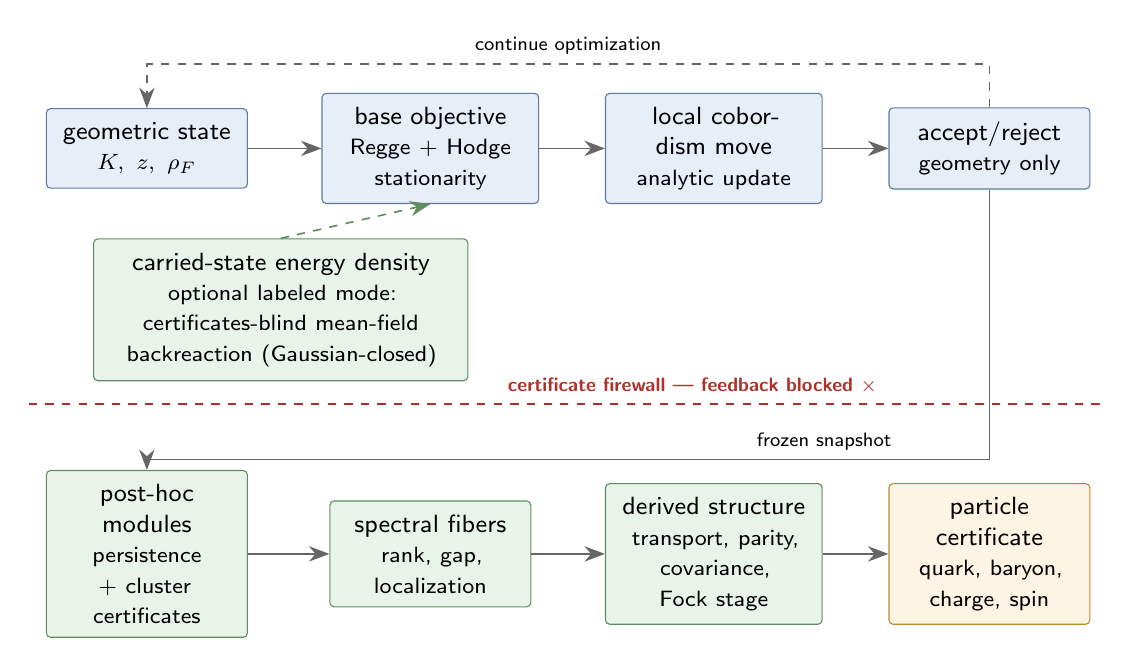
\begin{tikzpicture}
  % top row: geometry loop
  \node[estbox,text width=22mm] (geo)    at (0,0)    {geometric state\\ \footnotesize $K,\ z,\ \rho_{F}$};
  \node[estbox,text width=24mm] (obj)    at (3.6,0)  {base objective\\ \footnotesize Regge $+$ Hodge stationarity};
  \node[estbox,text width=24mm] (move)   at (7.2,0)  {local cobordism move\\ \footnotesize analytic update};
  \node[estbox,text width=22mm] (accept) at (10.7,0) {accept/reject\\ \footnotesize geometry only};
  \draw[flow] (geo) -- (obj);
  \draw[flow] (obj) -- (move);
  \draw[flow] (move) -- (accept);
  \draw[flow,dashed] (accept.north) -- ++(0,0.55) -| (geo.north)
    node[pos=0.25,above,font=\scriptsize\sffamily]{continue optimization};
  % optional backreaction (labeled mode)
  \node[derivbox,text width=44mm] (backr) at (1.7,-2.05)
    {carried-state energy density\\ \footnotesize optional labeled mode: certificates-blind mean-field backreaction (Gaussian-closed)};
  \draw[flow,dashed,draw=derivgreenline] (backr.north) -- (obj.south);
  % firewall
  \draw[dashed,thick,firewallred] (-1.5,-3.25) -- (12.1,-3.25)
    node[pos=0.62,above,font=\scriptsize\sffamily\bfseries,color=firewallred]
      {certificate firewall --- feedback blocked $\times$};
  % bottom row
  \node[derivbox,text width=22mm] (post) at (0,-5.15)   {post-hoc modules\\ \footnotesize persistence $+$ cluster certificates};
  \node[derivbox,text width=22mm] (fib)  at (3.6,-5.15) {spectral fibers\\ \footnotesize rank, gap, localization};
  \node[derivbox,text width=24mm] (der)  at (7.2,-5.15) {derived structure\\ \footnotesize transport, parity, covariance, Fock stage};
  \node[propbox,text width=22mm]  (cert) at (10.7,-5.15){particle certificate\\ \footnotesize quark, baryon, charge, spin};
  \draw[flow] (post) -- (fib);
  \draw[flow] (fib) -- (der);
  \draw[flow] (der) -- (cert);
  % frozen snapshot, crossing downward only
  \draw[flow] (accept.south) -- (10.7,-3.95) -- (0,-3.95) -- (post.north);
  \node[font=\scriptsize\sffamily] at (8.6,-3.72) {frozen snapshot};
\end{tikzpicture}
\caption{No-feedback emergence protocol. Only the base geometric objective
drives optimization. In the certificates-blind backreaction mode the carried
state's energy density may enter that objective;
Section~\ref{sec:quasifree} records that this remains inside the quasi-free
class. Cluster, fiber, color, exchange, and baryon observables are computed
from accepted snapshots and cannot feed back into the objective in either
emergence mode. Targeted synthesis is a separate, explicitly labeled mode.}
\label{fig:firewall}
\end{figure}

% ================================================================ 14
\section{The master recursive construction}\label{sec:master}

Let $\RN_{0}(\lambda)=L_{0}-\lambda I$ denote the microscopic one-particle
response pencil. At every scale:
\begin{equation*}
\boxed{
\begin{aligned}
  P_{\ell} &= \mathrm{PersistentPartition}(\RN_{\ell}),\\
  E_{v}^{\ell+1} &= \text{certified isolated subspace of } C_{v}^{\ell},\\
  \RN_{\ell+1}(\lambda) &= \mathrm{Feshbach}_{P_{\ell}}(\RN_{\ell}(\lambda)),\\
  V_{vw}^{\ell+1} &= \mathrm{Polar}_{r_{v}}
    \bigl((\Phi_{v}^{\ell})^{\dagger}WT_{vw}\Phi_{w}^{\ell}\bigr),\\
  \hh_{\ell+1} &= \lsum_{v}E_{v}^{\ell+1},\qquad
    J_{\ell+1}:\hh_{\ell+1}\to C(K),\qquad
    G_{\ell+1}=J_{\ell+1}^{\dagger}WJ_{\ell+1},\\
  \HK_{\ell+1} &= \Fock\bigl(\hh_{\ell+1}\bigr),
\end{aligned}}
\end{equation*}
where $\lsum$ is the abstract labeled sum: one summand per retained fiber, with
no claim that the geometric subspaces are independent inside $C(K)$.

The geometric subspaces $E_{v}\subset C(K)$ of adjacent components may overlap
on shared interface cells, so their internal sum need not be direct. The
recursion therefore never asserts $\bigoplus_{v}E_{v}\subset C(K)$. It forms
the abstract labeled sum, carries the embedding $J_{\ell+1}$ and its Gram
matrix $G_{\ell+1}$ exactly, and proceeds by exactly one of three declared
options: carry $G$ in every subsequent formula; certify
$\lVert G-I\rVert\le\varepsilon$ and propagate $\varepsilon$ through the
composable amplitude budget of Section~\ref{sec:interactions}; or quotient
$\ker G$ and restate the fiber ranks. A sheaf-stalk decomposition that assigns
interface modes to link stalks is a valid realization of the same requirement
\cite{hansenghrist2019}, but it is not necessary.

At $\lambda=0$ the response step is the exact supported static Schur
complement. For a nonzero band it is the exact energy-dependent pencil; a
cached linear $\RN_{\ell+1}$ is an AMLS/component-mode surrogate with a
declared frequency window and residual. The transport rank is generic; only an
anchored accepted rank-three fiber receives the color interpretation. This
recursion supplies the response network, retained stalk, derived transport, and
expanding state space without claiming that every coarse level is literally a
new simplicial complex.

% ================================================================ 15
\section{Exactness and performance principles}\label{sec:performance}

The simulation should prefer an exact structural identity over a general dense
numerical operation whenever both compute the same object:
\begin{itemize}
  \item in the quasi-free sector, evolve the covariance matrix by
    $i\dot{\Gamma}=[h,\Gamma]$ and evaluate every polynomial certificate by
    Wick contraction; materialize a Fock vector only for oracle tests or
    explicitly non-Gaussian boundary data;
  \item use sparse static and shifted Schur/Feshbach solves, not explicit dense
    inverses, and use AMLS when a reusable linear band surrogate is needed;
  \item use K\"unneth sums only for actual product complexes, and occupation
    subset sums for $\dG(L)$, not diagonalization of an eager Fock matrix;
  \item use exterior bit parity for exchange signs, not sampled phases;
  \item use exact $3\times 3$ determinants and the fixed $F_{3}$ frame only
    after a rank-three band passes its triangle-anchor certificate;
  \item use analytic Regge/Hodge derivatives and Wirtinger gradients, not
    finite differences;
  \item use Smith normal form for integer homology and a spectral threshold
    only as a cross-check;
  \item use matrix-determinant/Woodbury updates for local cobordism changes;
  \item cache component factorizations and invalidate only affected stars;
  \item keep tensor products lazy and block-sparse by occupation/parity;
  \item use $U(r)$ polar transport at generic rank, retaining determinant-line
    and projective/center data at $r=3$; and
  \item attach frequency window, residual, gap, leakage, signature, and
    condition-number certificates to every iterative eigensolve or reduction.
\end{itemize}

The exact route is not only faster. It prevents a numerical tolerance from
becoming an undocumented physical postulate.

% ================================================================ 16
\section{Prior art and boundary of novelty}\label{sec:priorart}

No single cited work establishes the full recursive spectral-fiber proposal.
The construction is a synthesis of several mature ideas, and its novelty should
be evaluated at the joins. Table~\ref{tab:priorart} states the boundary
explicitly.

\begingroup\small
\setlength{\tabcolsep}{5pt}
\setlength{\LTleft}{0pt}\setlength{\LTright}{0pt}
\begin{longtable}{p{0.2\linewidth}p{0.36\linewidth}p{0.36\linewidth}}
\caption{Established ingredients and the additional Tessera claim.}
\label{tab:priorart}\\
\toprule
Topic & Established prior art & Additional claim made here\\
\midrule
\endfirsthead
\toprule
Topic & Established prior art & Additional claim made here\\
\midrule
\endhead
\midrule
\multicolumn{3}{r}{\footnotesize continued on next page}\\
\endfoot
\bottomrule
\endlastfoot
Simplicial geometry and Hodge spectra &
Regge curvature, discrete exterior calculus, and combinatorial Laplace spectra
\cite{regge1961,dec2005,horakjost2013}. &
Use one jointly optimized Regge--Hodge complex as the only microscopic carrier
for geometry and quantum readouts.\\
\addlinespace
Coarse response and recursive modules &
Kron/Schur reduction, Feshbach maps, component-mode synthesis/AMLS, cellular
sheaf Laplacians, modular communities, and self-similar network
renormalization
\cite{craigbampton1968,bennighoflehoucq2004,bcfs2003,dorflerbullo2013,%
hansenghrist2019,reichardtbornholdt2006,songhavlin2005,fortunatobarthelemy2007}. &
Treat a persistent component as a static response vertex; retain nonzero bands
through shifted or certified component-mode reduction; recurse in
operator-valued response networks, using a sheaf realization only when its
factorization is certified.\\
\addlinespace
Quasi-free many-body calculus &
Second quantization, generalized Hartree--Fock theory, and quasi-free/Gaussian
state methods \cite{berezin1966,bls1994}. &
Run the entire particle-certificate layer on the covariance matrix; prove
mean-field geometry backreaction is Gaussian-closed; treat sharp-certificate
failure as a structural dichotomy rather than a numerical shortfall.\\
\addlinespace
Geometric gauge transport &
Berry and Wilczek--Zee holonomy, overlap-based lattice links, connection
Laplacians/vector diffusion, and Wilson loops
\cite{berry1984,wilczekzee1984,fukui2005,wilson1974,singerwu2012}. &
Derive $U(r)$ transport from component frames; at anchored rank three retain
the determinant line, projective $SU(3)/\mathbb{Z}_{3}$ class, and any chosen
center lift, assigning no independent gauge link variable.\\
\addlinespace
Color and fermion structure &
Quark/color triplets, exterior Fock/second quantization, topological exchange
phases, and spin structures
\cite{gellmann1964,hannambu1965,greenberg1964,berezin1966,%
laidlawdewitt1971,leinaasmyrheim1977,lawsonmichelsohn1989,%
cimasonireshetikhin2007}. &
Realize $\mathbf{1}\oplus\mathbf{3}\oplus\overline{\mathbf{3}}\oplus\mathbf{1}$
on three oriented edge modes, anchor abstract rank-three fibers to oriented
faces, and test exchange by a Berry-cancelled determinant-line interferometer
plus structural permutation parity.\\
\addlinespace
Scale composition and boundaries &
TQFT cobordisms, general-boundary state assignments, categorical tensor
composition, second quantization, and entanglement renormalization
\cite{atiyah1988,oeckl2003,abramskycoecke2004,berezin1966,vidal2007}. &
Keep simplicial gluing at the one-particle level, then build finite Fock stages
functorially and require vacuum-embedding compatibility under refinement.\\
\addlinespace
K\"ahler--Dirac boundary &
Differential-form fermions and their taste structure
\cite{becherjoos1982,buttcatterall2021}. &
Do not infer K\"ahler--Dirac tastes from occupation exterior algebra; test for
them only if the one-particle field is promoted to inhomogeneous cochains with
a K\"ahler--Dirac operator.\\
\addlinespace
Spectral spacetime &
Diffusion spectral dimension on ensembles of simplicial geometries
\cite{ajl2005}. &
Test whether many interacting Tessera cobordisms yield a stable
four-dimensional spectral window while simultaneously supporting the particle
certificates.\\
\end{longtable}
\endgroup

\begin{figure}[htb]
\centering
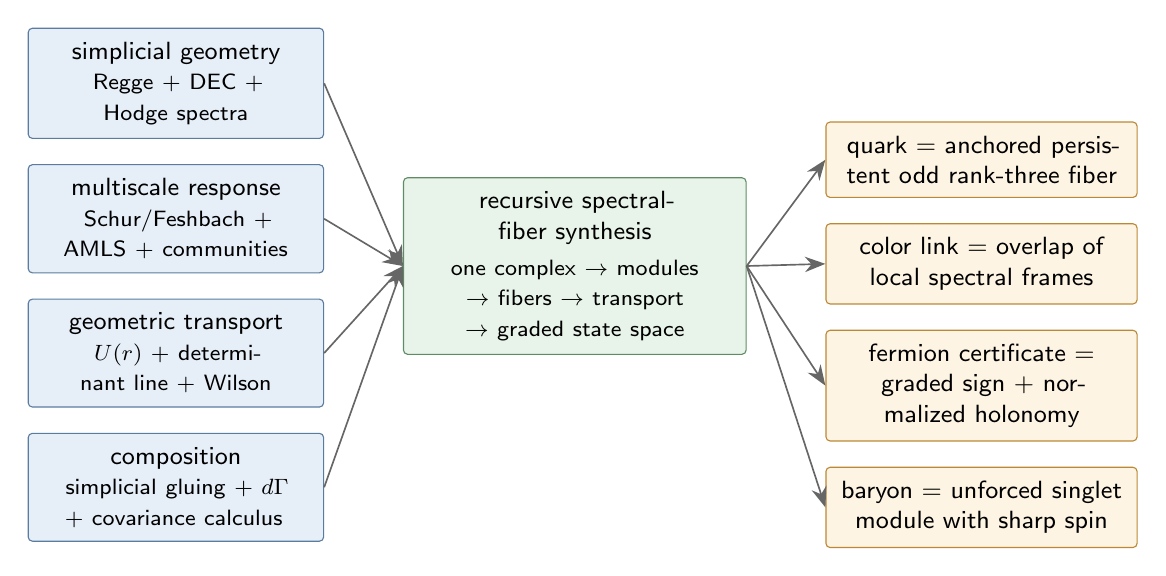
\begin{tikzpicture}[node distance=3.2mm and 10mm]
  \node[estbox,text width=34mm] (in1) {simplicial geometry\\ \footnotesize Regge $+$ DEC $+$ Hodge spectra};
  \node[estbox,text width=34mm,below=of in1] (in2) {multiscale response\\ \footnotesize Schur/Feshbach $+$ AMLS $+$ communities};
  \node[estbox,text width=34mm,below=of in2] (in3) {geometric transport\\ \footnotesize $U(r)$ $+$ determinant line $+$ Wilson};
  \node[estbox,text width=34mm,below=of in3] (in4) {composition\\ \footnotesize simplicial gluing $+$ $\dG$ $+$ covariance calculus};
  \node[derivbox,text width=40mm,right=of in2,yshift=-6mm] (core)
    {recursive spectral-fiber synthesis\\[2pt]\footnotesize one complex $\to$ modules $\to$ fibers $\to$ transport $\to$ graded state space};
  \node[propbox,text width=36mm,right=of core,yshift=13.5mm] (o1) {quark $=$ anchored persistent odd rank-three fiber};
  \node[propbox,text width=36mm,below=of o1] (o2) {color link $=$ overlap of local spectral frames};
  \node[propbox,text width=36mm,below=of o2] (o3) {fermion certificate $=$ graded sign $+$ normalized holonomy};
  \node[propbox,text width=36mm,below=of o3] (o4) {baryon $=$ unforced singlet module with sharp spin};
  \draw[flow] (in1.east) -- (core.west);
  \draw[flow] (in2.east) -- (core.west);
  \draw[flow] (in3.east) -- (core.west);
  \draw[flow] (in4.east) -- (core.west);
  \draw[flow] (core.east) -- (o1.west);
  \draw[flow] (core.east) -- (o2.west);
  \draw[flow] (core.east) -- (o3.west);
  \draw[flow] (core.east) -- (o4.west);
\end{tikzpicture}
\caption{Relationship to prior art. The blue inputs are established research
programs; the green center is the proposed Tessera synthesis; the amber outputs
are new physical identifications and must be validated independently. An arrow
denotes conceptual inheritance, not a proof of the downstream claim.}
\label{fig:priorart}
\end{figure}

% ================================================================ 17
\section{Falsification program}\label{sec:falsification}

The formulation fails, or must be narrowed, if any of the following persists
under refinement and tighter numerical certification:
\begin{enumerate}
  \item \textbf{No persistent rank-three clusters.} Certified components
    appear, but their localized fiber rank or spectral gap is unstable.
  \item \textbf{No oriented color anchor.} A rank-three band appears, but its
    calibrated anchor profile (Section~\ref{sec:quarks}) vanishes or drifts.
  \item \textbf{No faithful coarse response.} Schur-reduced components fail to
    reproduce static response, or shifted/AMLS reduction fails over its
    declared frequency band, within the stated residual.
  \item \textbf{No derived gauge covariance.} Wilson values depend on the local
    spectral frame after leakage is controlled, or the determinant and
    $\mathbb{Z}_{3}$ center sectors cannot be made path-consistent.
  \item \textbf{No fermion holonomy.} The Berry-cancelled exchange ratio or
    structural permutation sign does not give \code{-1}, or the verdict
    changes under relabeling.
  \item \textbf{No spinor rotation.} Exchange works but the
    reference-normalized $2\pi$ physical rotation does not give \code{-1}; in
    a manifold-like continuum claim, failure of a consistent spin lift is also
    decisive.
  \item \textbf{No inductive compatibility.} Adding vacuum modes changes
    already-computed amplitudes by a nonvanishing amount.
  \item \textbf{No quasi-free proton.} Every other certificate is met inside
    the covariance-only theory, but $\operatorname{Var}(J^{2})$ fails to
    converge to zero on every accepted candidate across refinement. This
    outcome is a branch point rather than a refutation of the geometry: it
    mandates adopting exactly one of the non-Gaussian mechanisms of
    Section~\ref{sec:quasifree}, as an explicit scope decision, before any
    proton claim is made.
  \item \textbf{No unforced baryon.} Targeted synthesis can build the
    certificates, but the stationary geometric ensemble never produces them
    without a proton-specific term.
  \item \textbf{No continuum stability.} Dimensionless color, parity, charge,
    spin, and amplitude certificates drift rather than converge with
    refinement.
  \item \textbf{Unexpected multiplicity.} A robust flavor/taste degeneracy is
    neither predicted by the stated one-particle operator nor stable enough to
    be promoted to an emergent flavor mechanism.
\end{enumerate}

Holes may re-emerge and may correlate with some phases, but no claim in this
paper depends on them doing so.

% ================================================================ 18
\section{Conclusion}\label{sec:conclusion}

The geometry is economical and precise: an edge carries a two-level mode, not
an independently stored pure state; a quark candidate is a modular spectral
component whose rank-three band is anchored to oriented faces by a calibrated
profile; its transport is a certified $U(3)$ overlap with retained
determinant-line and projective color data; and its fermionic sign is the
exterior grading, checked dynamically only after cancelling ordinary Berry
phase. Simplicial gluing constructs the one-particle operator and second
quantization constructs the expanding Fock state. Three accepted components
form a baryon through their normalized color wedge; the proton is the sharpest
test because it also demands the correct determinant-line flux, charge, flavor,
and a variance-certified spin response.

The exact claims are limited to their proper domains: static Schur response,
energy-dependent Feshbach isospectrality, exterior/CAR algebra,
second-quantized direct-sum composition, gauge covariance of accepted
transport, and closure of the quasi-free class under every generator the model
currently possesses. That last identity organizes the programme. Classical or
mean-field geometry backreaction does not leave the Gaussian manifold, so the
covariance matrix is not an approximation tier: it is the exact state
representation of the present theory, and every \emph{polynomial} certificate
on it --- including $\langle J^{2}\rangle$ and its variance --- is a finite Wick
sum. The certificates that are not polynomial in the mode operators --- the
determinant winding, the Gauss flux, the rotation character, the spin lift, the
anchor, and the crossing readouts of Section~\ref{sec:readout} --- are read from
geometry and holonomy instead, and are no less exact for it.

What remains genuinely open is whether Tessera's unforced Regge--Hodge dynamics
produces the required anchored clusters, low-leakage holonomies, relative
determinant windings, and sharp spin response. A tempting
Hellmann--Feynman/envelope argument does not by itself make the first variation
of transport Gram defect vanish at a Regge--Hodge stationary point, because the
defect is not the optimized functional; Tessera will therefore measure that
correlation as a conjectural scaling law rather than cite stationarity as a
theorem. The decisive question is the dichotomy of
Section~\ref{sec:quasifree}: either an exact covariance-only proton exists, or
a genuinely non-Gaussian, geometry-mediated interaction is required. Either
outcome is a result. The first makes the particle layer exactly and
polynomially certifiable; the second would be the first internal evidence that
the geometry must supply a true interaction term, through one of the five
mechanisms this paper names.

% ================================================================ refs
\renewcommand{\refname}{Prior-art references}
\phantomsection
\addcontentsline{toc}{section}{Prior-art references}
\begin{thebibliography}{33}
\small

\bibitem{ajl2005}
Jan Ambj\o rn, Jerzy Jurkiewicz, and Renate Loll.
Spectral dimension of the universe.
\emph{Physical Review Letters}, 95:171301, 2005.
doi:10.1103/PhysRevLett.95.171301.
URL \url{https://arxiv.org/abs/hep-th/0505113}.

\bibitem{regge1961}
Tullio Regge.
General relativity without coordinates.
\emph{Il Nuovo Cimento}, 19:558--571, 1961.
doi:10.1007/BF02733251.

\bibitem{dec2005}
Mathieu Desbrun, Anil N. Hirani, Melvin Leok, and Jerrold E. Marsden.
Discrete exterior calculus, 2005.
URL \url{https://arxiv.org/abs/math/0508341}.

\bibitem{horakjost2013}
Danijela Horak and J\"urgen Jost.
Spectra of combinatorial laplace operators on simplicial complexes.
\emph{Advances in Mathematics}, 244:303--336, 2013.
doi:10.1016/j.aim.2013.05.005.
URL \url{https://arxiv.org/abs/1105.2712}.

\bibitem{craigbampton1968}
Roy R. Craig~Jr. and Mervyn C. C. Bampton.
Coupling of substructures for dynamic analyses.
\emph{AIAA Journal}, 6(7):1313--1319, 1968.
doi:10.2514/3.4741.

\bibitem{bennighoflehoucq2004}
Jeffrey K. Bennighof and Richard B. Lehoucq.
An automated multilevel substructuring method for eigenspace computation in
linear elastodynamics.
\emph{SIAM Journal on Scientific Computing}, 25(6):2084--2106, 2004.

\bibitem{bcfs2003}
Volker Bach, Thomas Chen, J\"urg Fr\"ohlich, and Israel Michael Sigal.
Smooth feshbach map and operator-theoretic renormalization group methods.
\emph{Journal of Functional Analysis}, 203(1):44--92, 2003.
doi:10.1016/S0022-1236(03)00057-0.

\bibitem{dorflerbullo2013}
Florian D\"orfler and Francesco Bullo.
Kron reduction of graphs with applications to electrical networks.
\emph{IEEE Transactions on Circuits and Systems I: Regular Papers},
60(1):150--163, 2013.
doi:10.1109/TCSI.2012.2215780.
URL \url{https://arxiv.org/abs/1102.2950}.

\bibitem{loukas2019}
Andreas Loukas.
Graph reduction with spectral and cut guarantees.
\emph{Journal of Machine Learning Research}, 20(116):1--42, 2019.
URL \url{https://jmlr.org/papers/v20/18-680.html}.

\bibitem{hansenghrist2019}
Jakob Hansen and Robert Ghrist.
Toward a spectral theory of cellular sheaves.
\emph{Journal of Applied and Computational Topology}, 3:315--358, 2019.
doi:10.1007/s41468-019-00038-7.
URL \url{https://arxiv.org/abs/1808.01513}.

\bibitem{reichardtbornholdt2006}
J\"org Reichardt and Stefan Bornholdt.
Statistical mechanics of community detection.
\emph{Physical Review E}, 74:016110, 2006.
doi:10.1103/PhysRevE.74.016110.

\bibitem{songhavlin2005}
Chaoming Song, Shlomo Havlin, and Hern\'an A. Makse.
Self-similarity of complex networks.
\emph{Nature}, 433:392--395, 2005.
doi:10.1038/nature03248.

\bibitem{fortunatobarthelemy2007}
Santo Fortunato and Marc Barth\'elemy.
Resolution limit in community detection.
\emph{Proceedings of the National Academy of Sciences}, 104(1):36--41, 2007.
doi:10.1073/pnas.0605965104.
URL \url{https://arxiv.org/abs/physics/0607100}.

\bibitem{berezin1966}
Felix A. Berezin.
\emph{The Method of Second Quantization}.
Academic Press, New York, 1966.

\bibitem{atiyah1988}
Michael F. Atiyah.
Topological quantum field theories.
\emph{Publications Math\'ematiques de l'IH\'ES}, 68:175--186, 1988.
doi:10.1007/BF02698547.

\bibitem{oeckl2003}
Robert Oeckl.
A ``general boundary'' formulation for quantum mechanics and quantum gravity.
\emph{Physics Letters B}, 575:318--324, 2003.
doi:10.1016/j.physletb.2003.08.043.
URL \url{https://arxiv.org/abs/hep-th/0306025}.

\bibitem{abramskycoecke2004}
Samson Abramsky and Bob Coecke.
A categorical semantics of quantum protocols.
In \emph{Proceedings of the 19th Annual IEEE Symposium on Logic in Computer
Science}, pages 415--425, 2004.
doi:10.1109/LICS.2004.1319636.
URL \url{https://arxiv.org/abs/quant-ph/0402130}.

\bibitem{bls1994}
Volker Bach, Elliott H. Lieb, and Jan Philip Solovej.
Generalized Hartree--Fock theory and the Hubbard model.
\emph{Journal of Statistical Physics}, 76(1--2):3--89, 1994.
doi:10.1007/BF02188656.

\bibitem{cimasonireshetikhin2007}
David Cimasoni and Nicolai Reshetikhin.
Dimers on surface graphs and spin structures. i.
\emph{Communications in Mathematical Physics}, 275:187--208, 2007.
doi:10.1007/s00220-007-0302-7.

\bibitem{gellmann1964}
Murray Gell-Mann.
A schematic model of baryons and mesons.
\emph{Physics Letters}, 8(3):214--215, 1964.
doi:10.1016/S0031-9163(64)92001-3.

\bibitem{hannambu1965}
Moo-Young Han and Yoichiro Nambu.
Three-triplet model with double SU(3) symmetry.
\emph{Physical Review}, 139:B1006--B1010, 1965.
doi:10.1103/PhysRev.139.B1006.

\bibitem{greenberg1964}
O. W. Greenberg.
Spin and unitary-spin independence in a paraquark model of baryons and mesons.
\emph{Physical Review Letters}, 13:598--602, 1964.
doi:10.1103/PhysRevLett.13.598.

\bibitem{berry1984}
Michael V. Berry.
Quantal phase factors accompanying adiabatic changes.
\emph{Proceedings of the Royal Society of London A}, 392(1802):45--57, 1984.
doi:10.1098/rspa.1984.0023.

\bibitem{wilczekzee1984}
Frank Wilczek and A. Zee.
Appearance of gauge structure in simple dynamical systems.
\emph{Physical Review Letters}, 52:2111--2114, 1984.
doi:10.1103/PhysRevLett.52.2111.

\bibitem{fukui2005}
Takahiro Fukui, Yasuhiro Hatsugai, and Hiroshi Suzuki.
Chern numbers in discretized brillouin zone: Efficient method of computing
(spin) hall conductances.
\emph{Journal of the Physical Society of Japan}, 74(6):1674--1677, 2005.
doi:10.1143/JPSJ.74.1674.
URL \url{https://arxiv.org/abs/cond-mat/0503172}.

\bibitem{wilson1974}
Kenneth G. Wilson.
Confinement of quarks.
\emph{Physical Review D}, 10:2445--2459, 1974.
doi:10.1103/PhysRevD.10.2445.

\bibitem{lawsonmichelsohn1989}
H. Blaine Lawson~Jr. and Marie-Louise Michelsohn.
\emph{Spin Geometry}.
Princeton University Press, Princeton, 1989.

\bibitem{laidlawdewitt1971}
Michael G. G. Laidlaw and C\'ecile Morette DeWitt.
Feynman functional integrals for systems of indistinguishable particles.
\emph{Physical Review D}, 3:1375--1378, 1971.
doi:10.1103/PhysRevD.3.1375.

\bibitem{leinaasmyrheim1977}
Jon M. Leinaas and Jan Myrheim.
On the theory of identical particles.
\emph{Il Nuovo Cimento B}, 37:1--23, 1977.
doi:10.1007/BF02727953.

\bibitem{vidal2007}
Guifr\'e Vidal.
Entanglement renormalization.
\emph{Physical Review Letters}, 99:220405, 2007.
doi:10.1103/PhysRevLett.99.220405.
URL \url{https://arxiv.org/abs/cond-mat/0512165}.

\bibitem{becherjoos1982}
Peter Becher and Hans Joos.
The dirac--k\"ahler equation and fermions on the lattice.
\emph{Zeitschrift f\"ur Physik C}, 15:343--365, 1982.
doi:10.1007/BF01614426.

\bibitem{buttcatterall2021}
Nouman Butt, Simon Catterall, Arnab Pradhan, and Goksu Can Toga.
Anomalies and symmetric mass generation for k\"ahler--dirac fermions.
\emph{Physical Review D}, 104:094504, 2021.
doi:10.1103/PhysRevD.104.094504.
URL \url{https://arxiv.org/abs/2101.01026}.

\bibitem{singerwu2012}
Amit Singer and Hau-Tieng Wu.
Vector diffusion maps and the connection laplacian.
\emph{Communications on Pure and Applied Mathematics}, 65(8):1067--1144, 2012.
doi:10.1002/cpa.21395.
URL \url{https://arxiv.org/abs/1102.0075}.

\end{thebibliography}

% ================================================================ repo
\section*{Repository evidence}
\addcontentsline{toc}{section}{Repository evidence}

\begin{itemize}
  \item Tessera amplitude and obstruction results, \code{cobordism-results.md}.
  \item Tessera spectral-dimension status, \code{h\_ds4\_status.md}.
  \item Tessera interaction-history construction,
    \code{interaction-history-monte-carlo.md}.
  \item Existing total-space spin obstruction,
    \code{joint\_proton\_spin\_findings.md}.
  \item Existing fixed-partition modularity implementation,
    \code{ModularityOptimizer.h}.
  \item Current visualization and joint-stationarity experiment,
    \code{proton\_animation.py}.
  \item External-review dispositions and exact-claim ledger, review rounds one
    and two, \code{referee response}.
\end{itemize}

\end{document}
